\documentclass[]{article}
\usepackage{lmodern}
\usepackage{amssymb,amsmath}
\usepackage{ifxetex,ifluatex}
\usepackage{fixltx2e} % provides \textsubscript
\ifnum 0\ifxetex 1\fi\ifluatex 1\fi=0 % if pdftex
  \usepackage[T1]{fontenc}
  \usepackage[utf8]{inputenc}
\else % if luatex or xelatex
  \ifxetex
    \usepackage{mathspec}
  \else
    \usepackage{fontspec}
  \fi
  \defaultfontfeatures{Ligatures=TeX,Scale=MatchLowercase}
\fi
% use upquote if available, for straight quotes in verbatim environments
\IfFileExists{upquote.sty}{\usepackage{upquote}}{}
% use microtype if available
\IfFileExists{microtype.sty}{%
\usepackage{microtype}
\UseMicrotypeSet[protrusion]{basicmath} % disable protrusion for tt fonts
}{}
\usepackage[margin=1in]{geometry}
\usepackage{hyperref}
\hypersetup{unicode=true,
            pdftitle={ANCOVA},
            pdfauthor={Walter Gruber},
            pdfborder={0 0 0},
            breaklinks=true}
\urlstyle{same}  % don't use monospace font for urls
\usepackage{color}
\usepackage{fancyvrb}
\newcommand{\VerbBar}{|}
\newcommand{\VERB}{\Verb[commandchars=\\\{\}]}
\DefineVerbatimEnvironment{Highlighting}{Verbatim}{commandchars=\\\{\}}
% Add ',fontsize=\small' for more characters per line
\usepackage{framed}
\definecolor{shadecolor}{RGB}{248,248,248}
\newenvironment{Shaded}{\begin{snugshade}}{\end{snugshade}}
\newcommand{\KeywordTok}[1]{\textcolor[rgb]{0.13,0.29,0.53}{\textbf{#1}}}
\newcommand{\DataTypeTok}[1]{\textcolor[rgb]{0.13,0.29,0.53}{#1}}
\newcommand{\DecValTok}[1]{\textcolor[rgb]{0.00,0.00,0.81}{#1}}
\newcommand{\BaseNTok}[1]{\textcolor[rgb]{0.00,0.00,0.81}{#1}}
\newcommand{\FloatTok}[1]{\textcolor[rgb]{0.00,0.00,0.81}{#1}}
\newcommand{\ConstantTok}[1]{\textcolor[rgb]{0.00,0.00,0.00}{#1}}
\newcommand{\CharTok}[1]{\textcolor[rgb]{0.31,0.60,0.02}{#1}}
\newcommand{\SpecialCharTok}[1]{\textcolor[rgb]{0.00,0.00,0.00}{#1}}
\newcommand{\StringTok}[1]{\textcolor[rgb]{0.31,0.60,0.02}{#1}}
\newcommand{\VerbatimStringTok}[1]{\textcolor[rgb]{0.31,0.60,0.02}{#1}}
\newcommand{\SpecialStringTok}[1]{\textcolor[rgb]{0.31,0.60,0.02}{#1}}
\newcommand{\ImportTok}[1]{#1}
\newcommand{\CommentTok}[1]{\textcolor[rgb]{0.56,0.35,0.01}{\textit{#1}}}
\newcommand{\DocumentationTok}[1]{\textcolor[rgb]{0.56,0.35,0.01}{\textbf{\textit{#1}}}}
\newcommand{\AnnotationTok}[1]{\textcolor[rgb]{0.56,0.35,0.01}{\textbf{\textit{#1}}}}
\newcommand{\CommentVarTok}[1]{\textcolor[rgb]{0.56,0.35,0.01}{\textbf{\textit{#1}}}}
\newcommand{\OtherTok}[1]{\textcolor[rgb]{0.56,0.35,0.01}{#1}}
\newcommand{\FunctionTok}[1]{\textcolor[rgb]{0.00,0.00,0.00}{#1}}
\newcommand{\VariableTok}[1]{\textcolor[rgb]{0.00,0.00,0.00}{#1}}
\newcommand{\ControlFlowTok}[1]{\textcolor[rgb]{0.13,0.29,0.53}{\textbf{#1}}}
\newcommand{\OperatorTok}[1]{\textcolor[rgb]{0.81,0.36,0.00}{\textbf{#1}}}
\newcommand{\BuiltInTok}[1]{#1}
\newcommand{\ExtensionTok}[1]{#1}
\newcommand{\PreprocessorTok}[1]{\textcolor[rgb]{0.56,0.35,0.01}{\textit{#1}}}
\newcommand{\AttributeTok}[1]{\textcolor[rgb]{0.77,0.63,0.00}{#1}}
\newcommand{\RegionMarkerTok}[1]{#1}
\newcommand{\InformationTok}[1]{\textcolor[rgb]{0.56,0.35,0.01}{\textbf{\textit{#1}}}}
\newcommand{\WarningTok}[1]{\textcolor[rgb]{0.56,0.35,0.01}{\textbf{\textit{#1}}}}
\newcommand{\AlertTok}[1]{\textcolor[rgb]{0.94,0.16,0.16}{#1}}
\newcommand{\ErrorTok}[1]{\textcolor[rgb]{0.64,0.00,0.00}{\textbf{#1}}}
\newcommand{\NormalTok}[1]{#1}
\usepackage{longtable,booktabs}
\usepackage{graphicx,grffile}
\makeatletter
\def\maxwidth{\ifdim\Gin@nat@width>\linewidth\linewidth\else\Gin@nat@width\fi}
\def\maxheight{\ifdim\Gin@nat@height>\textheight\textheight\else\Gin@nat@height\fi}
\makeatother
% Scale images if necessary, so that they will not overflow the page
% margins by default, and it is still possible to overwrite the defaults
% using explicit options in \includegraphics[width, height, ...]{}
\setkeys{Gin}{width=\maxwidth,height=\maxheight,keepaspectratio}
\IfFileExists{parskip.sty}{%
\usepackage{parskip}
}{% else
\setlength{\parindent}{0pt}
\setlength{\parskip}{6pt plus 2pt minus 1pt}
}
\setlength{\emergencystretch}{3em}  % prevent overfull lines
\providecommand{\tightlist}{%
  \setlength{\itemsep}{0pt}\setlength{\parskip}{0pt}}
\setcounter{secnumdepth}{5}
% Redefines (sub)paragraphs to behave more like sections
\ifx\paragraph\undefined\else
\let\oldparagraph\paragraph
\renewcommand{\paragraph}[1]{\oldparagraph{#1}\mbox{}}
\fi
\ifx\subparagraph\undefined\else
\let\oldsubparagraph\subparagraph
\renewcommand{\subparagraph}[1]{\oldsubparagraph{#1}\mbox{}}
\fi

%%% Use protect on footnotes to avoid problems with footnotes in titles
\let\rmarkdownfootnote\footnote%
\def\footnote{\protect\rmarkdownfootnote}

%%% Change title format to be more compact
\usepackage{titling}

% Create subtitle command for use in maketitle
\newcommand{\subtitle}[1]{
  \posttitle{
    \begin{center}\large#1\end{center}
    }
}

\setlength{\droptitle}{-2em}

  \title{ANCOVA}
    \pretitle{\vspace{\droptitle}\centering\huge}
  \posttitle{\par}
    \author{Walter Gruber}
    \preauthor{\centering\large\emph}
  \postauthor{\par}
      \predate{\centering\large\emph}
  \postdate{\par}
    \date{2019-03-26}


\begin{document}
\maketitle

{
\setcounter{tocdepth}{2}
\tableofcontents
}
\section*{Vorbemerkung}\label{vorbemerkung}
\addcontentsline{toc}{section}{Vorbemerkung}

Dieses Skriptum wurde mit dem Paket \emph{bookdown} erstellt. Der
verwendete R-Code wird als Teil des Skriptums angeführt und kann auch
direkt von diesem Dokument in ein R-Skript übernommen und ausgeführt
werden. Erläuterungen zum Code beschränken sich zum Teil auf wesentliche
Code-Fragmente. Für detaillierte Angaben zu diversen Funktionen ist die
R-Hilfe zu verwenden.

Der nachfolgende Code ist spezifisch für die Erstellung dieses
Dokumentes, sowie der Bearbeitung der Beispiele im Kurs von Bedeutung.
Es wird in diesem Code-Teil sichergestellt, dass die verwendeten Pakte
vorhanden und geladen sind. Daher sollte dieser Code am Anfang jeder
neuen R-Datei übernommen werden. Die Vorgehensweise ist:

\begin{enumerate}
\def\labelenumi{\arabic{enumi}.}
\tightlist
\item
  Starten von R-Studio
\item
  Öffnen einer neuen R-Script Datei
\item
  Kopiere die nachfolgenden Zeilen in diese Datei
\item
  Speichere die Datei mit einem entsprechenden Namen
\item
  Führe diesen Code aus
\item
  Füge deinen Code nach diesen Zeilen ein
\end{enumerate}

\begin{Shaded}
\begin{Highlighting}[]
\CommentTok{# Initialisierung}
\KeywordTok{rm}\NormalTok{(}\DataTypeTok{list =} \KeywordTok{ls}\NormalTok{())}
\ControlFlowTok{if}\NormalTok{ (}\OperatorTok{!}\KeywordTok{require}\NormalTok{(}\StringTok{"pacman"}\NormalTok{)) }\KeywordTok{install.packages}\NormalTok{(}\StringTok{"pacman"}\NormalTok{)}
\NormalTok{pacman}\OperatorTok{::}\KeywordTok{p_load}\NormalTok{(corrplot, DAAG, dataMaid, devtools, doBy, DT, }
\NormalTok{               ggformula, ggplot2, gridExtra, htmlwidgets, }
\NormalTok{               imager, knitr, labelled, leaps, magick, MASS, }
\NormalTok{               NHANES, mosaic, mosaicCore, mosaicData, pander,}
\NormalTok{               pastecs, ppcor, reshape2, }
\NormalTok{               rockchalk, rpart, rpart.plot)}
\end{Highlighting}
\end{Shaded}

Des Weiteren ist es von Vorteil, zu Beginn einer Auswertung/Datenanalyse
mit R eine entsprechende Verzeichnisstruktur im Window-Dateimanager
festzulegen und für diese Struktur ein R-Projektfile anzulegen. Die
Verzeichnisstruktur richtet sich im Allgemeinen nach der jeweiligen
Analyse, folgende Vorgaben haben sich aber bereits schon mehrmals
bewährt:

\begin{figure}
\centering
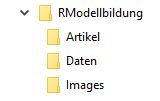
\includegraphics[width=0.20000\textwidth]{Images/Verzeichnisstruktur.JPG}
\caption{\textbf{Abbildung 1}: Dateistruktur für R-Projekt}
\end{figure}

Die Root kann dabei entweder auf der lokalen Festplatte (C:/..) oder
einem Server, bzw. Cloud (../NextCloud/R Modellbildung/Images) liegen.

Das Anlegen eines R-Projektes wird im RStudio durchgeführt.

\begin{figure}
\centering
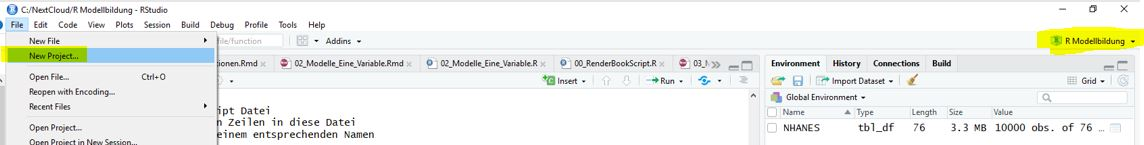
\includegraphics[width=1.00000\textwidth]{Images/Projektdefinieren.JPG}
\caption{\textbf{Abbildung 2}: R-Projekt definieren}
\end{figure}

Nachdem bereits eine Verzeichnisstruktur definiert wurde, kann man das
Projekt in das bereits definierte Verzeichnis legen (Folge den Schritten
die von RStudio vorgegeben werden). Den Vorteil des projektbasierten
Arbeitens werden wir im Verlauf des Kurses noch näher kennen lernen.

Inhalte, Beispiele und Daten stammen teilweise aus dem Internet, u.a.
(Coursera \protect\hyperlink{ref-CourseRa}{2018}), (DataCamp
\protect\hyperlink{ref-DataCamp}{2018}) und den Büchern (Field
\protect\hyperlink{ref-Field}{2017}), (Bühner
\protect\hyperlink{ref-Buehner1}{2009}) und (Bühner
\protect\hyperlink{ref-Buehner2}{2017}).

\section*{Motivation}\label{motivation}
\addcontentsline{toc}{section}{Motivation}

Die Kovarianzanalyse (ANCOVA) ist ein Spezialfall der ANOVA. Beide
werden verwendet, um die Auswirkungen kategorischer Variablen (Faktoren)
auf eine intervall- oder ratio-level abhängige Variable zu testen.

Die ANCOVA gibt uns jedoch die zusätzliche Möglichkeit, gleichzeitig die
Wirkung anderer kontinuierlicher Variablen auf die abhängige Variable zu
beurteilen oder zu kontrollieren. Kontinuierliche Variablen, die als
Unabhängige in einem ANOVA-Design enthalten sind und die mit einer
abhängigen Variablen kovariabel sind, nennt man \emph{Kovariablen}.

Bei der ANCOVA geht es im Wesentlichen darum, die Fehlervarianz bei
randomisierten Gruppenexperimenten weiter zu verringern.

ANCOVA wird jedoch häufiger eingesetzt, wenn eine Randomisierung nicht
möglich ist. In diesen Fällen müssen wir uns oft mit so genannten
``nicht-äquivalenten'' (nicht zufällig zugeordneten) Gruppen zufrieden
geben. Per Definition können sich solche Gruppen in erheblicher Weise
unterscheiden, auch bei Merkmalen, die die Ergebnisvariable beeinflussen
können. Solange sie nicht berücksichtigt werden, kann das Vorhandensein
dieser Hintergrund- oder Fremdvariablen die Fehlervarianz erhöhen,
unseren ``Signal-Rausch-Abstand'' verringern und es letztendlich
schwieriger machen, einen echten Unterschied zwischen den Gruppen zu
erkennen.

\section*{Kovarianzanalyse}\label{kovarianzanalyse}
\addcontentsline{toc}{section}{Kovarianzanalyse}

Im folgenden betrachten wir ein Beispiel, welches die Auswirkungen von
Viagra auf den Libido untersucht.

Es ist naheliegend anzunehmen, dass auch andere Faktoren (wie andere
Medikamente, Müdigkeit, etc.) den Libido beeinflussen. Wenn diese
Variablen (die Kovariablen) gemessen werden, ist es möglich, den
Einfluss, den sie auf die abhängige Variable haben, durch Einbeziehung
in das Regressionsmodell zu steuern/kontrolliern.

Ziel ist es, den Effekt der Kovariaten auf die Zielvariable zu
\emph{entfernen}. Durch diese Maßnahme sollte sich die Wirkungsweise der
unabhängigen Variablen (Viagra) auf den Libodo \emph{besser} zeigen. Es
gibt im Wesentlichen zwei Gründe\footnote{Es gibt noch andere Gründe für
  die Aufnahme von Kovariablen in die ANOVA, welche in der Berechnung
  der ANCOVA detailliert beschrieben werden. Siehe (Stevens
  \protect\hyperlink{ref-Stevens}{2002}), (Wildt
  \protect\hyperlink{ref-Wildt}{2009}).} für die Aufnahme von
Kovariablen in die ANOVA:

\begin{itemize}
\item
  \textbf{Reduzierung der Fehlervarianz}: in der ANOVA und beim t-Tests
  wird die Wirkung eines Experiments anhand der erklärbaren Variabilität
  in den Daten, mit der nicht erklärbaren Variabiliät verglichen. Wenn
  ein Teil dieser \emph{unerklärten} Varianz (\emph{SSR}) einer anderen
  Variablen (\emph{Kovariablen}) zugeordnet werden kann, reduziert sich
  die Fehlervarianz. Damit kann die Wirkung der unabhängigen Variable
  (\emph{SSM}) genauer beurteilt werden.
\item
  \textbf{Eliminierung von Confounds}: in jedem Experiment kann/wird es
  Variablen geben, welche nicht gemessen/erhoben wurden, die aber die
  Ergebnisse der Zielvariablen durchaus beeinflussen können. Sind diese
  bekannt, kann mit Hilfe der ANCOVA dieser Einfluss beseitigt werden.
\end{itemize}

Im vorliegenden Beispiel gehen wir davon aus, dass der Libido der
Sexualpartner den eigenen Libido beeinflusst\footnote{wie oft sie
  versuchten, sexuellen Kontakt aufzunehmen.}. Das entsprechende
Regressionsmodell erweitert sich demnach zu:

\(libido_i = b_0 + b_3 \cdot covariate_i + b_2 \cdot high_i + b_1 \cdot low_i + \varepsilon_i\)

\subsection*{Voraussetzungen}\label{voraussetzungen}
\addcontentsline{toc}{subsection}{Voraussetzungen}

Die ANCOVA hat die gleichen Annahmen wie ANOVA, zu welchen es jedoch
noch zwei wichtige zusätzliche Überlegungen gibt:

\begin{enumerate}
\def\labelenumi{\arabic{enumi}.}
\tightlist
\item
  \textbf{Unabhängigkeit von der Kovariablen- und dem Treatmenteffekt}.
  Abbildung \textbf{4-A} zeigt die bereits aus der ANOVA bekannte
  Zerlegung der Varianzen in eine Fehlervarianz und einer
  Treatmentvarianz. Abbildung \textbf{4-B} stellt eine ideale
  Voraussetzung für die Verwendung einer Kovariaten dar. Hierbei wird
  durch die Kovariate ein Teil der Fehlervarianz erklärt, ohne den
  Effekt des Treatment zu beeinflussen. Abbildung \textbf{4-C} hingegen
  zeigt das Problem bei einer fälschlicherweise verwendeten Kovariaten.
  Die Kovariate verringert zwar nach wir vor die Fehlervarianz, aber
  gleichzeitig wird auch der Treatmenteffekt beeinflusst. Statistisch
  gesehen können wir nur festhalten, dass die Kovariate und das
  Treatment Varianz gemeinsam erkären. Eine Trennung dieser gemeinsamen
  Varianz in Anteile Viagra und Kovariate ist nicht möglich! Eine
  einfache Möglichkeit die Kovariate auf ihre Eigenschaft zu prüfen, ist
  ein einfacher Mittelwertsvergleich (t-Test, ANOVA) der nach
  Viagragruppen aufgeteilten Kovariaten. Wenn die Gruppen sich nicht
  unterscheiden, kann von einer Unabhängigkeit ausgegangen werden und
  sofern die anderen Voraussetzungen erfüllt sind, die Kovariate
  verwendet werden. Auch durch eine Randomisierung der Gruppenzuordnung
  kann man unerwünschte Effekte (in Bezug auf die Wirkung der
  Kovariaten) zwischen den Gruppen evtl. vermeiden.
\end{enumerate}

\begin{figure}
\centering
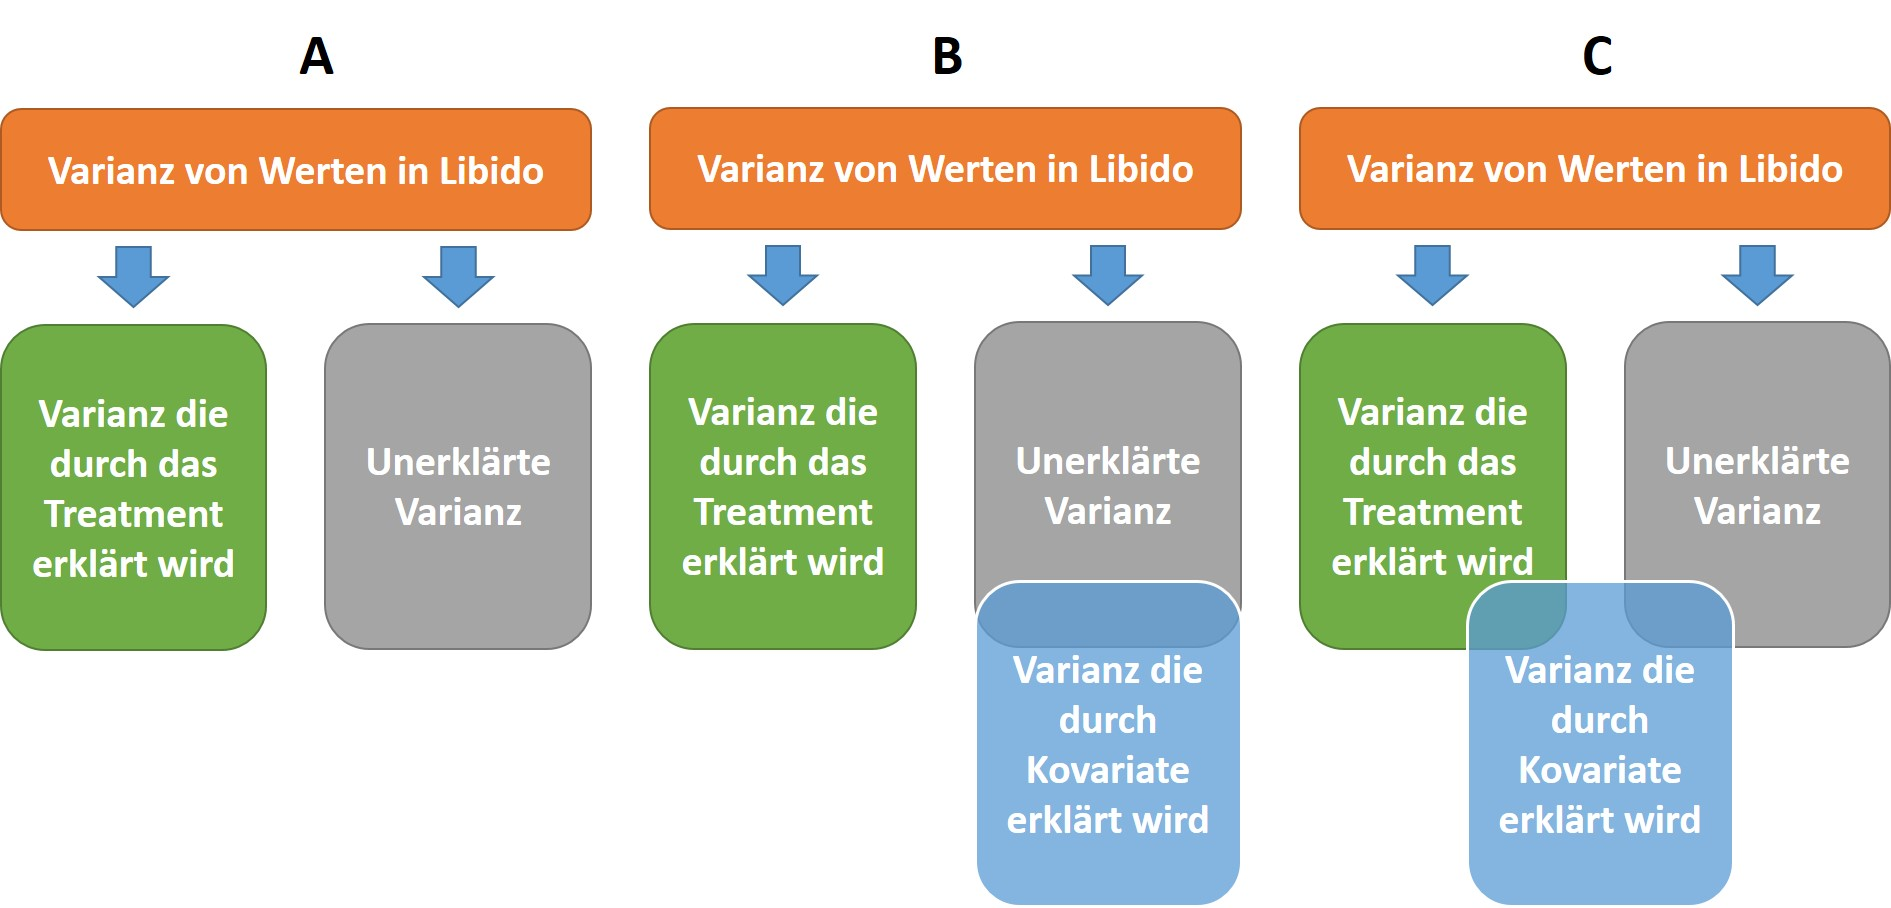
\includegraphics[width=0.80000\textwidth]{Images/Kovarianz_Field_11_2.jpg}
\caption{\textbf{Abbildung 4}: Wirkungsweise von Kovariate}
\end{figure}

Zum besseren Verständnis der mit den ANOVA-Verfahren verbundenen
Varianzaufteilung betrachten wir nochmals im Detail die Eigenschaften
der verschiedenen Varianzanteile.

Die Gesamtvarianz (im vorigen Graphen die Varianz von Werten im Libido)
wird folgendermaßen ermittelt:

\begin{figure}
\centering
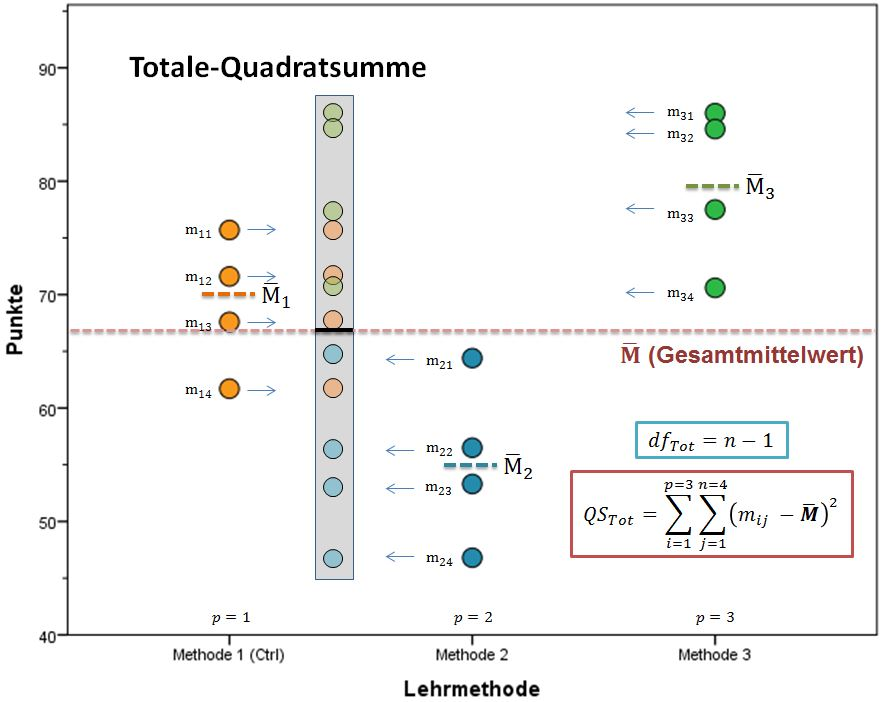
\includegraphics[width=0.80000\textwidth]{Images/ANOVA_QS_Total_Graphisch.jpg}
\caption{\textbf{Abbildung 5}: Totale Quadratsumme}
\end{figure}

Die Treatmentvarianz (im vorigen Graphen die Varianz die durch das
Treatment erklärt wird) entspricht der Variabilität der Mittelwerte der
jeweiligen Gruppen (in unserem Fall der Dosierungsstufen):

\begin{figure}
\centering
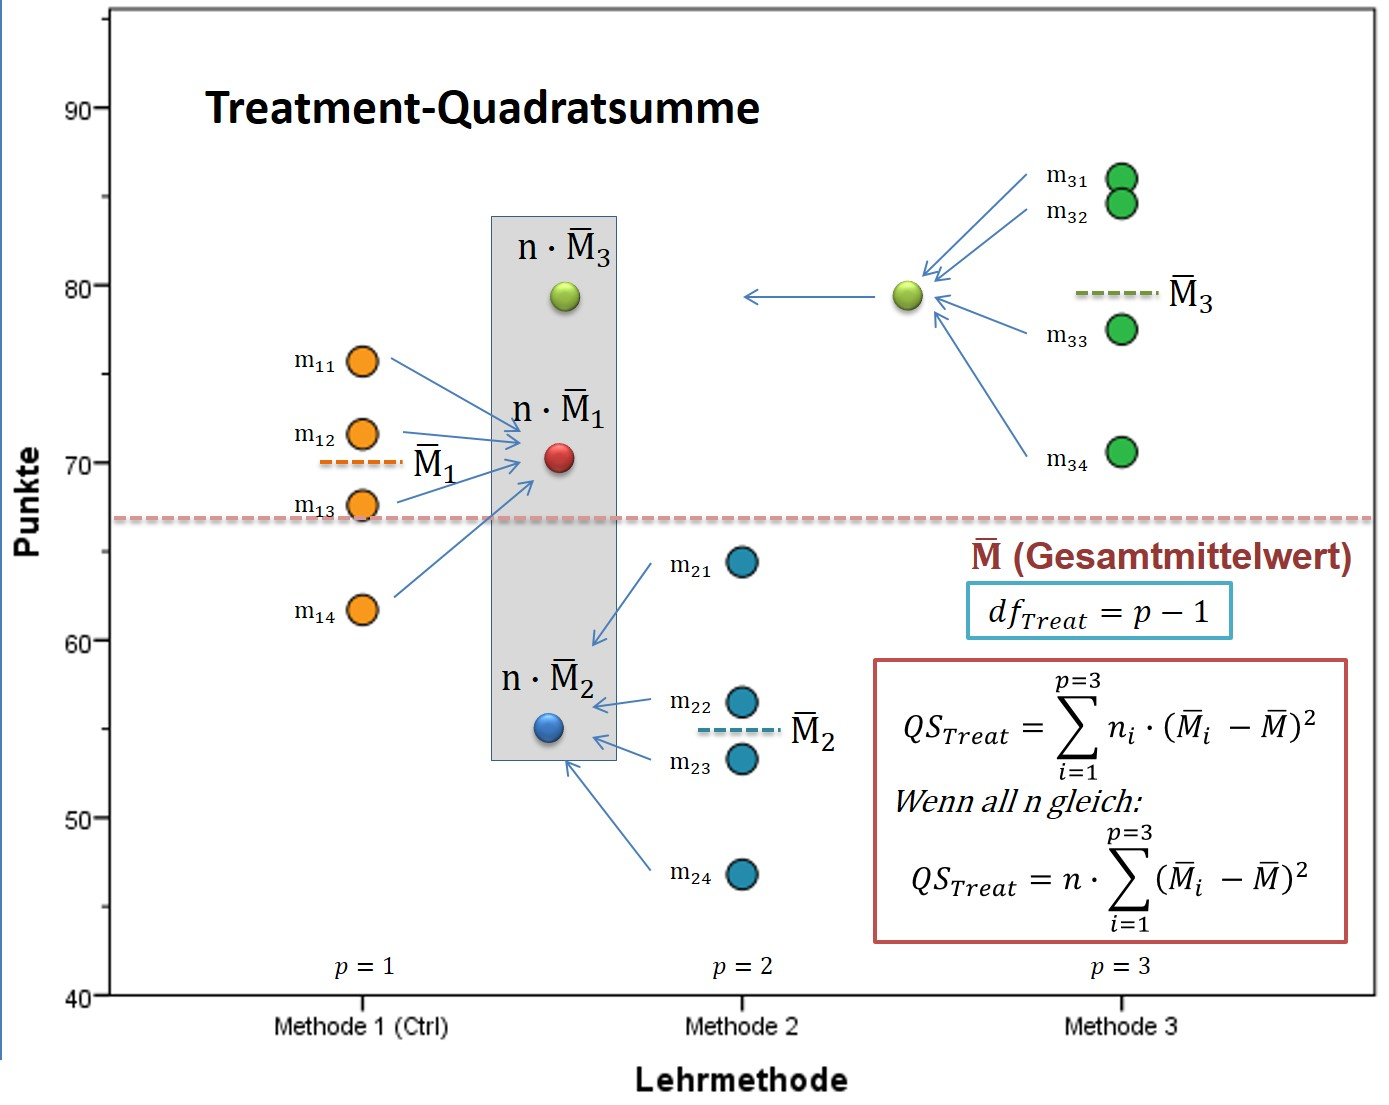
\includegraphics[width=0.80000\textwidth]{Images/ANOVA_QS_Treatment_Graphisch.jpg}
\caption{\textbf{Abbildung 6}: Treatmentquadratsumme}
\end{figure}

Die Fehlervarianz wird aus den durchschnittlichen Abweichungen der
beobachteten Werte zu den jeweiligen Gruppenmittelwerten bestimmt
(geschätzt). Anhand dieser Darstellung wird auch klar, warum die
Varianzgleichheit über die Gruppen hinweg gleich sein sollte. Wäre das
nämlich nicht gegeben, würde die Additivität (\(QS_1 + \cdots + QS_k\)
nicht gegeben sein.

\begin{figure}
\centering
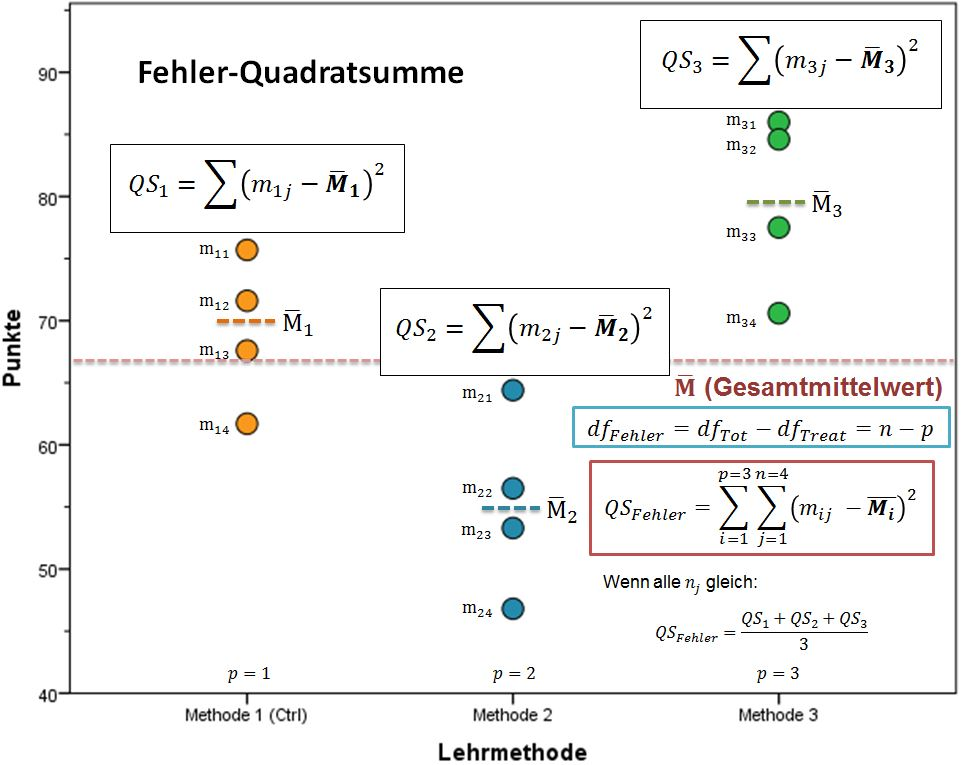
\includegraphics[width=0.80000\textwidth]{Images/ANOVA_QS_Fehler_Graphisch.jpg}
\caption{\textbf{Abbildung 7}: Fehlerquadratsumme}
\end{figure}

\begin{enumerate}
\def\labelenumi{\arabic{enumi}.}
\setcounter{enumi}{1}
\tightlist
\item
  \textbf{Homogenität der Regressionssteigungen}. Bei einer ANCOVA wird
  die Gesamtbeziehung zwischen dem Ergebnis (abhängige Variable) und der
  Kovariablen analysiert. D.h., es wird eine \emph{Regressionslinie an
  den gesamten Datensatz angepasst} und man \emph{ignoriert, zu welcher
  Gruppe eine Person gehört}. Bei der Anpassung dieses Gesamtmodells
  gehen wir daher davon aus, dass diese Gesamtbeziehung für alle
  Teilnehmergruppen gilt. Diese Annahme ist für die ANCOVA sehr wichtig.
  Der beste Weg diese Annahme zu kontrollieren, ist eine Darstellung der
  Kovariablen (\emph{Partner's Libido}) auf der einen und dem Ergebnis
  (\emph{Libido}) auf der anderen Achse, getrennt nach den Gruppen
  (\emph{Dosierung}). Die Regressionslinien sollten dann mehr oder
  weniger gleich aussehen (d.h. die Werte von \(b\) in jeder Gruppe
  sollten gleich sein). Im nachfolgender Darstellung wäre diese
  Voraussetung nicht erfüllt!
\end{enumerate}

\begin{figure}
\centering
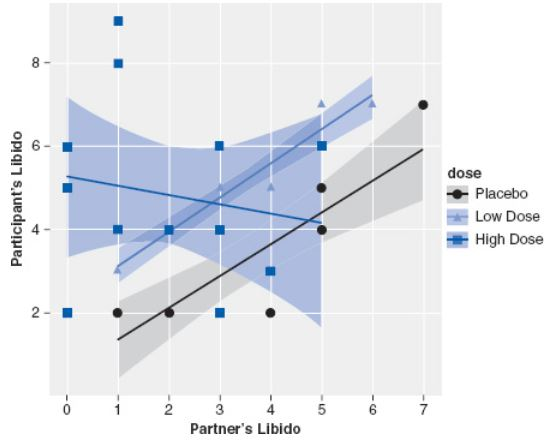
\includegraphics[width=0.60000\textwidth]{Images/Kovarianz_Field_11_3.jpg}
\caption{\textbf{Abbildung 8}: Verletzung der Homogenitätsbedingung}
\end{figure}

\subsection*{Berechnung einer ANCOVA}\label{berechnung-einer-ancova}
\addcontentsline{toc}{subsection}{Berechnung einer ANCOVA}

Bei der Berechnung einer ANCOVA sollten folgende Schritte durchgeführt
werden:

\begin{enumerate}
\def\labelenumi{\arabic{enumi}.}
\tightlist
\item
  Grafischen Darstellung der Daten und der Berechnung einiger
  deskriptiver Statistiken. Dabei sollten auch die Verteilungsannahmen
  überprüfen und den Levene-Test durchgeführt werden (Homogenitätstest).
\item
  Überprüfen der Kovariable und alle unabhängigen Variablen auf
  Unabhängigkeit, d.h. eine ANOVA mit der Kovariablen als Ergebnis und
  alle unabhängigen Variablen als Prädiktoren durchführen. Damit wird
  sichergestellt, dass sich die Kovariable auf den Ebenen dieser
  Variablen nicht signifikant unterscheidet. Wenn man ein signifikantes
  Ergebnis erhält, dann ist die Analyse bei diesem Schritt
  beendet\footnote{möglicherweise kann man eine robuste Version des
    Tests ausführen, Details später.}.
\item
  Durchführen der ANCOVA.
\item
  Berechnung der \emph{Kontraste} oder \emph{post hoc-Tests} (falls
  signifikante Ergebnisse vorliegen).
\item
  Überprüfen der Homogenität der Regressionssteigungen. Dies kann
  graphisch (siehe oben) durchgeführt werden, oder man kann auch die
  ANCOVA erneut ausführen und die Interaktion zwischen der unabhängigen
  Variable und der Kovariablen ins Modell aufnehmen. Wenn diese
  Interaktion signifikant ist, kann man nicht von einer Homogenität der
  Regressionsflanken ausgehen!
\end{enumerate}

\subsubsection*{Deskriptive, graphisch und
Homogenität}\label{deskriptive-graphisch-und-homogenitat}
\addcontentsline{toc}{subsubsection}{Deskriptive, graphisch und
Homogenität}

Um die Verteilung von Daten darzustellen, kann man z.B. Boxplots für
\emph{Libido} als auch für \emph{Libido des Partners} erzeugen. Darüber
hinaus ist es hilfreich, die Beziehung zwischen der Ergebnisvariablen
und der Kovariablen innerhalb jeder Gruppe zu betrachten (dies sagt uns
etwas über die Homogenität der Steigungen aus).

\begin{center}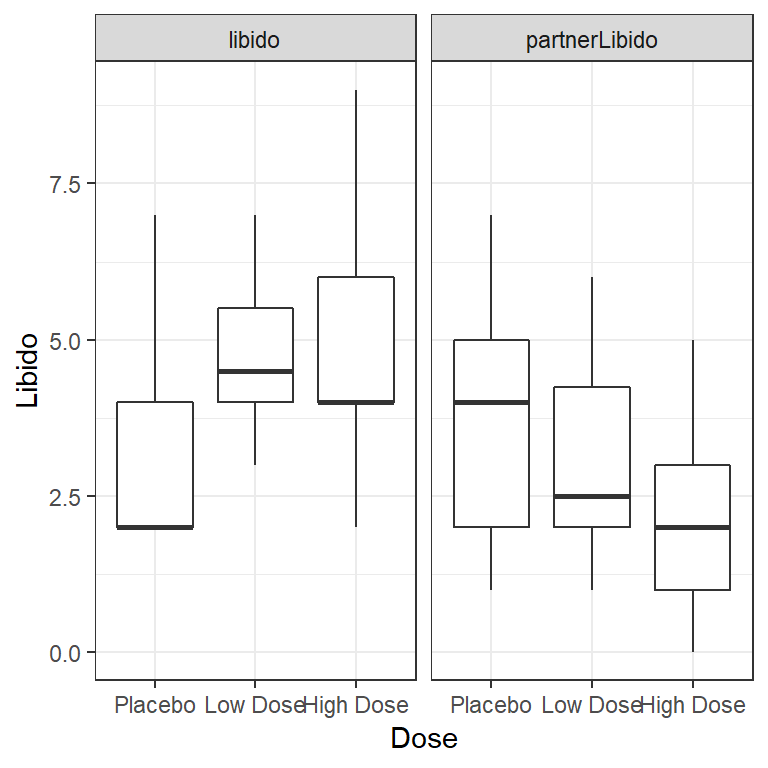
\includegraphics{01_ANCOVA_files/figure-latex/ANCOVA1-1} \end{center}

Die Boxplots zeigen den Libido bei den Teilnehmern und ihren Partnern
über die drei Dosen von Viagra. Die Libido scheint für die Teilnehmer
mit zunehmender Dosis von Viagra zu steigen, aber das Gegenteil gilt für
ihre Partner.

Neben der graphischen Darstellung sind auch die deskriptiven Werte
aufschlussreich, da diese Kennwerte wie die Streung (\(sd\)) und
Mittelwerte (\(\bar{x}\)), Konfidenzintervalle (\(CI\)), etc. ausgegeben
werden.

\begin{longtable}[]{@{}ccccccc@{}}
\toprule
\begin{minipage}[b]{0.10\columnwidth}\centering\strut
median\strut
\end{minipage} & \begin{minipage}[b]{0.09\columnwidth}\centering\strut
mean\strut
\end{minipage} & \begin{minipage}[b]{0.11\columnwidth}\centering\strut
SE.mean\strut
\end{minipage} & \begin{minipage}[b]{0.17\columnwidth}\centering\strut
CI.mean.0.95\strut
\end{minipage} & \begin{minipage}[b]{0.09\columnwidth}\centering\strut
var\strut
\end{minipage} & \begin{minipage}[b]{0.11\columnwidth}\centering\strut
std.dev\strut
\end{minipage} & \begin{minipage}[b]{0.11\columnwidth}\centering\strut
coef.var\strut
\end{minipage}\tabularnewline
\midrule
\endhead
\begin{minipage}[t]{0.10\columnwidth}\centering\strut
2\strut
\end{minipage} & \begin{minipage}[t]{0.09\columnwidth}\centering\strut
3.222\strut
\end{minipage} & \begin{minipage}[t]{0.11\columnwidth}\centering\strut
0.5958\strut
\end{minipage} & \begin{minipage}[t]{0.17\columnwidth}\centering\strut
1.374\strut
\end{minipage} & \begin{minipage}[t]{0.09\columnwidth}\centering\strut
3.194\strut
\end{minipage} & \begin{minipage}[t]{0.11\columnwidth}\centering\strut
1.787\strut
\end{minipage} & \begin{minipage}[t]{0.11\columnwidth}\centering\strut
0.5547\strut
\end{minipage}\tabularnewline
\bottomrule
\end{longtable}

\begin{longtable}[]{@{}ccccccc@{}}
\toprule
\begin{minipage}[b]{0.10\columnwidth}\centering\strut
median\strut
\end{minipage} & \begin{minipage}[b]{0.09\columnwidth}\centering\strut
mean\strut
\end{minipage} & \begin{minipage}[b]{0.11\columnwidth}\centering\strut
SE.mean\strut
\end{minipage} & \begin{minipage}[b]{0.17\columnwidth}\centering\strut
CI.mean.0.95\strut
\end{minipage} & \begin{minipage}[b]{0.09\columnwidth}\centering\strut
var\strut
\end{minipage} & \begin{minipage}[b]{0.11\columnwidth}\centering\strut
std.dev\strut
\end{minipage} & \begin{minipage}[b]{0.11\columnwidth}\centering\strut
coef.var\strut
\end{minipage}\tabularnewline
\midrule
\endhead
\begin{minipage}[t]{0.10\columnwidth}\centering\strut
4.5\strut
\end{minipage} & \begin{minipage}[t]{0.09\columnwidth}\centering\strut
4.875\strut
\end{minipage} & \begin{minipage}[t]{0.11\columnwidth}\centering\strut
0.5154\strut
\end{minipage} & \begin{minipage}[t]{0.17\columnwidth}\centering\strut
1.219\strut
\end{minipage} & \begin{minipage}[t]{0.09\columnwidth}\centering\strut
2.125\strut
\end{minipage} & \begin{minipage}[t]{0.11\columnwidth}\centering\strut
1.458\strut
\end{minipage} & \begin{minipage}[t]{0.11\columnwidth}\centering\strut
0.299\strut
\end{minipage}\tabularnewline
\bottomrule
\end{longtable}

\begin{longtable}[]{@{}ccccccc@{}}
\toprule
\begin{minipage}[b]{0.10\columnwidth}\centering\strut
median\strut
\end{minipage} & \begin{minipage}[b]{0.09\columnwidth}\centering\strut
mean\strut
\end{minipage} & \begin{minipage}[b]{0.11\columnwidth}\centering\strut
SE.mean\strut
\end{minipage} & \begin{minipage}[b]{0.17\columnwidth}\centering\strut
CI.mean.0.95\strut
\end{minipage} & \begin{minipage}[b]{0.09\columnwidth}\centering\strut
var\strut
\end{minipage} & \begin{minipage}[b]{0.11\columnwidth}\centering\strut
std.dev\strut
\end{minipage} & \begin{minipage}[b]{0.11\columnwidth}\centering\strut
coef.var\strut
\end{minipage}\tabularnewline
\midrule
\endhead
\begin{minipage}[t]{0.10\columnwidth}\centering\strut
4\strut
\end{minipage} & \begin{minipage}[t]{0.09\columnwidth}\centering\strut
4.846\strut
\end{minipage} & \begin{minipage}[t]{0.11\columnwidth}\centering\strut
0.5867\strut
\end{minipage} & \begin{minipage}[t]{0.17\columnwidth}\centering\strut
1.278\strut
\end{minipage} & \begin{minipage}[t]{0.09\columnwidth}\centering\strut
4.474\strut
\end{minipage} & \begin{minipage}[t]{0.11\columnwidth}\centering\strut
2.115\strut
\end{minipage} & \begin{minipage}[t]{0.11\columnwidth}\centering\strut
0.4365\strut
\end{minipage}\tabularnewline
\bottomrule
\end{longtable}

\begin{longtable}[]{@{}ccccccc@{}}
\toprule
\begin{minipage}[b]{0.10\columnwidth}\centering\strut
median\strut
\end{minipage} & \begin{minipage}[b]{0.09\columnwidth}\centering\strut
mean\strut
\end{minipage} & \begin{minipage}[b]{0.11\columnwidth}\centering\strut
SE.mean\strut
\end{minipage} & \begin{minipage}[b]{0.17\columnwidth}\centering\strut
CI.mean.0.95\strut
\end{minipage} & \begin{minipage}[b]{0.09\columnwidth}\centering\strut
var\strut
\end{minipage} & \begin{minipage}[b]{0.11\columnwidth}\centering\strut
std.dev\strut
\end{minipage} & \begin{minipage}[b]{0.11\columnwidth}\centering\strut
coef.var\strut
\end{minipage}\tabularnewline
\midrule
\endhead
\begin{minipage}[t]{0.10\columnwidth}\centering\strut
4\strut
\end{minipage} & \begin{minipage}[t]{0.09\columnwidth}\centering\strut
3.444\strut
\end{minipage} & \begin{minipage}[t]{0.11\columnwidth}\centering\strut
0.6894\strut
\end{minipage} & \begin{minipage}[t]{0.17\columnwidth}\centering\strut
1.59\strut
\end{minipage} & \begin{minipage}[t]{0.09\columnwidth}\centering\strut
4.278\strut
\end{minipage} & \begin{minipage}[t]{0.11\columnwidth}\centering\strut
2.068\strut
\end{minipage} & \begin{minipage}[t]{0.11\columnwidth}\centering\strut
0.6005\strut
\end{minipage}\tabularnewline
\bottomrule
\end{longtable}

\begin{longtable}[]{@{}ccccccc@{}}
\toprule
\begin{minipage}[b]{0.10\columnwidth}\centering\strut
median\strut
\end{minipage} & \begin{minipage}[b]{0.09\columnwidth}\centering\strut
mean\strut
\end{minipage} & \begin{minipage}[b]{0.11\columnwidth}\centering\strut
SE.mean\strut
\end{minipage} & \begin{minipage}[b]{0.17\columnwidth}\centering\strut
CI.mean.0.95\strut
\end{minipage} & \begin{minipage}[b]{0.09\columnwidth}\centering\strut
var\strut
\end{minipage} & \begin{minipage}[b]{0.11\columnwidth}\centering\strut
std.dev\strut
\end{minipage} & \begin{minipage}[b]{0.11\columnwidth}\centering\strut
coef.var\strut
\end{minipage}\tabularnewline
\midrule
\endhead
\begin{minipage}[t]{0.10\columnwidth}\centering\strut
2.5\strut
\end{minipage} & \begin{minipage}[t]{0.09\columnwidth}\centering\strut
3.125\strut
\end{minipage} & \begin{minipage}[t]{0.11\columnwidth}\centering\strut
0.6105\strut
\end{minipage} & \begin{minipage}[t]{0.17\columnwidth}\centering\strut
1.444\strut
\end{minipage} & \begin{minipage}[t]{0.09\columnwidth}\centering\strut
2.982\strut
\end{minipage} & \begin{minipage}[t]{0.11\columnwidth}\centering\strut
1.727\strut
\end{minipage} & \begin{minipage}[t]{0.11\columnwidth}\centering\strut
0.5526\strut
\end{minipage}\tabularnewline
\bottomrule
\end{longtable}

\begin{longtable}[]{@{}ccccccc@{}}
\toprule
\begin{minipage}[b]{0.10\columnwidth}\centering\strut
median\strut
\end{minipage} & \begin{minipage}[b]{0.08\columnwidth}\centering\strut
mean\strut
\end{minipage} & \begin{minipage}[b]{0.11\columnwidth}\centering\strut
SE.mean\strut
\end{minipage} & \begin{minipage}[b]{0.17\columnwidth}\centering\strut
CI.mean.0.95\strut
\end{minipage} & \begin{minipage}[b]{0.09\columnwidth}\centering\strut
var\strut
\end{minipage} & \begin{minipage}[b]{0.11\columnwidth}\centering\strut
std.dev\strut
\end{minipage} & \begin{minipage}[b]{0.11\columnwidth}\centering\strut
coef.var\strut
\end{minipage}\tabularnewline
\midrule
\endhead
\begin{minipage}[t]{0.10\columnwidth}\centering\strut
2\strut
\end{minipage} & \begin{minipage}[t]{0.08\columnwidth}\centering\strut
2\strut
\end{minipage} & \begin{minipage}[t]{0.11\columnwidth}\centering\strut
0.4529\strut
\end{minipage} & \begin{minipage}[t]{0.17\columnwidth}\centering\strut
0.9868\strut
\end{minipage} & \begin{minipage}[t]{0.09\columnwidth}\centering\strut
2.667\strut
\end{minipage} & \begin{minipage}[t]{0.11\columnwidth}\centering\strut
1.633\strut
\end{minipage} & \begin{minipage}[t]{0.11\columnwidth}\centering\strut
0.8165\strut
\end{minipage}\tabularnewline
\bottomrule
\end{longtable}

\begin{longtable}[]{@{}ccccccc@{}}
\toprule
\begin{minipage}[b]{0.10\columnwidth}\centering\strut
median\strut
\end{minipage} & \begin{minipage}[b]{0.09\columnwidth}\centering\strut
mean\strut
\end{minipage} & \begin{minipage}[b]{0.11\columnwidth}\centering\strut
SE.mean\strut
\end{minipage} & \begin{minipage}[b]{0.17\columnwidth}\centering\strut
CI.mean.0.95\strut
\end{minipage} & \begin{minipage}[b]{0.09\columnwidth}\centering\strut
var\strut
\end{minipage} & \begin{minipage}[b]{0.11\columnwidth}\centering\strut
std.dev\strut
\end{minipage} & \begin{minipage}[b]{0.11\columnwidth}\centering\strut
coef.var\strut
\end{minipage}\tabularnewline
\midrule
\endhead
\begin{minipage}[t]{0.10\columnwidth}\centering\strut
4\strut
\end{minipage} & \begin{minipage}[t]{0.09\columnwidth}\centering\strut
4.367\strut
\end{minipage} & \begin{minipage}[t]{0.11\columnwidth}\centering\strut
0.3571\strut
\end{minipage} & \begin{minipage}[t]{0.17\columnwidth}\centering\strut
0.7304\strut
\end{minipage} & \begin{minipage}[t]{0.09\columnwidth}\centering\strut
3.826\strut
\end{minipage} & \begin{minipage}[t]{0.11\columnwidth}\centering\strut
1.956\strut
\end{minipage} & \begin{minipage}[t]{0.11\columnwidth}\centering\strut
0.448\strut
\end{minipage}\tabularnewline
\bottomrule
\end{longtable}

\begin{longtable}[]{@{}ccccccc@{}}
\toprule
\begin{minipage}[b]{0.10\columnwidth}\centering\strut
median\strut
\end{minipage} & \begin{minipage}[b]{0.09\columnwidth}\centering\strut
mean\strut
\end{minipage} & \begin{minipage}[b]{0.11\columnwidth}\centering\strut
SE.mean\strut
\end{minipage} & \begin{minipage}[b]{0.17\columnwidth}\centering\strut
CI.mean.0.95\strut
\end{minipage} & \begin{minipage}[b]{0.09\columnwidth}\centering\strut
var\strut
\end{minipage} & \begin{minipage}[b]{0.11\columnwidth}\centering\strut
std.dev\strut
\end{minipage} & \begin{minipage}[b]{0.11\columnwidth}\centering\strut
coef.var\strut
\end{minipage}\tabularnewline
\midrule
\endhead
\begin{minipage}[t]{0.10\columnwidth}\centering\strut
2.5\strut
\end{minipage} & \begin{minipage}[t]{0.09\columnwidth}\centering\strut
2.733\strut
\end{minipage} & \begin{minipage}[t]{0.11\columnwidth}\centering\strut
0.3388\strut
\end{minipage} & \begin{minipage}[t]{0.17\columnwidth}\centering\strut
0.6929\strut
\end{minipage} & \begin{minipage}[t]{0.09\columnwidth}\centering\strut
3.444\strut
\end{minipage} & \begin{minipage}[t]{0.11\columnwidth}\centering\strut
1.856\strut
\end{minipage} & \begin{minipage}[t]{0.11\columnwidth}\centering\strut
0.6789\strut
\end{minipage}\tabularnewline
\bottomrule
\end{longtable}

Der Test auf Varianzhomogeniät wird mit dem Levene's-Test durchgeführt.
Dabei zeigt sich der Test mit dem Median als zentraler Kennwert robuster
als die Schätzung durch den Mittelwert (\emph{Bemerkung}: man kann auch
das Verhältnis der größten zur kleinsten Varianz\footnote{Hartely's
  \(F_{max}\) variance ratio.} (aus deskriptiver Statistik) bilden und
in einer entsprechenden Tabelle auf Signifikanz prüfen).

\begin{longtable}[]{@{}cccc@{}}
\caption{Levene's Test for Homogeneity of Variance (center =
median)}\tabularnewline
\toprule
\begin{minipage}[b]{0.15\columnwidth}\centering\strut
~\strut
\end{minipage} & \begin{minipage}[b]{0.06\columnwidth}\centering\strut
Df\strut
\end{minipage} & \begin{minipage}[b]{0.12\columnwidth}\centering\strut
F value\strut
\end{minipage} & \begin{minipage}[b]{0.12\columnwidth}\centering\strut
Pr(\textgreater{}F)\strut
\end{minipage}\tabularnewline
\midrule
\endfirsthead
\toprule
\begin{minipage}[b]{0.15\columnwidth}\centering\strut
~\strut
\end{minipage} & \begin{minipage}[b]{0.06\columnwidth}\centering\strut
Df\strut
\end{minipage} & \begin{minipage}[b]{0.12\columnwidth}\centering\strut
F value\strut
\end{minipage} & \begin{minipage}[b]{0.12\columnwidth}\centering\strut
Pr(\textgreater{}F)\strut
\end{minipage}\tabularnewline
\midrule
\endhead
\begin{minipage}[t]{0.15\columnwidth}\centering\strut
\textbf{group}\strut
\end{minipage} & \begin{minipage}[t]{0.06\columnwidth}\centering\strut
2\strut
\end{minipage} & \begin{minipage}[t]{0.12\columnwidth}\centering\strut
0.3256\strut
\end{minipage} & \begin{minipage}[t]{0.12\columnwidth}\centering\strut
0.7249\strut
\end{minipage}\tabularnewline
\begin{minipage}[t]{0.15\columnwidth}\centering\strut
\strut
\end{minipage} & \begin{minipage}[t]{0.06\columnwidth}\centering\strut
27\strut
\end{minipage} & \begin{minipage}[t]{0.12\columnwidth}\centering\strut
NA\strut
\end{minipage} & \begin{minipage}[t]{0.12\columnwidth}\centering\strut
NA\strut
\end{minipage}\tabularnewline
\bottomrule
\end{longtable}

\begin{longtable}[]{@{}cccc@{}}
\caption{Levene's Test for Homogeneity of Variance (center =
mean)}\tabularnewline
\toprule
\begin{minipage}[b]{0.15\columnwidth}\centering\strut
~\strut
\end{minipage} & \begin{minipage}[b]{0.06\columnwidth}\centering\strut
Df\strut
\end{minipage} & \begin{minipage}[b]{0.12\columnwidth}\centering\strut
F value\strut
\end{minipage} & \begin{minipage}[b]{0.12\columnwidth}\centering\strut
Pr(\textgreater{}F)\strut
\end{minipage}\tabularnewline
\midrule
\endfirsthead
\toprule
\begin{minipage}[b]{0.15\columnwidth}\centering\strut
~\strut
\end{minipage} & \begin{minipage}[b]{0.06\columnwidth}\centering\strut
Df\strut
\end{minipage} & \begin{minipage}[b]{0.12\columnwidth}\centering\strut
F value\strut
\end{minipage} & \begin{minipage}[b]{0.12\columnwidth}\centering\strut
Pr(\textgreater{}F)\strut
\end{minipage}\tabularnewline
\midrule
\endhead
\begin{minipage}[t]{0.15\columnwidth}\centering\strut
\textbf{group}\strut
\end{minipage} & \begin{minipage}[t]{0.06\columnwidth}\centering\strut
2\strut
\end{minipage} & \begin{minipage}[t]{0.12\columnwidth}\centering\strut
0.7112\strut
\end{minipage} & \begin{minipage}[t]{0.12\columnwidth}\centering\strut
0.5\strut
\end{minipage}\tabularnewline
\begin{minipage}[t]{0.15\columnwidth}\centering\strut
\strut
\end{minipage} & \begin{minipage}[t]{0.06\columnwidth}\centering\strut
27\strut
\end{minipage} & \begin{minipage}[t]{0.12\columnwidth}\centering\strut
NA\strut
\end{minipage} & \begin{minipage}[t]{0.12\columnwidth}\centering\strut
NA\strut
\end{minipage}\tabularnewline
\bottomrule
\end{longtable}

\subsubsection*{Unabhängigkeit}\label{unabhangigkeit}
\addcontentsline{toc}{subsubsection}{Unabhängigkeit}

Die Unabhängigkeit kann man relativ einfach durch eine ANOVA mit
\emph{partnerLibido} als Ergebnis und \emph{Dosis} als Prädiktor
durchführen.

\begin{longtable}[]{@{}cccccc@{}}
\caption{Analysis of Variance Model}\tabularnewline
\toprule
\begin{minipage}[b]{0.19\columnwidth}\centering\strut
~\strut
\end{minipage} & \begin{minipage}[b]{0.06\columnwidth}\centering\strut
Df\strut
\end{minipage} & \begin{minipage}[b]{0.10\columnwidth}\centering\strut
Sum Sq\strut
\end{minipage} & \begin{minipage}[b]{0.12\columnwidth}\centering\strut
Mean Sq\strut
\end{minipage} & \begin{minipage}[b]{0.12\columnwidth}\centering\strut
F value\strut
\end{minipage} & \begin{minipage}[b]{0.12\columnwidth}\centering\strut
Pr(\textgreater{}F)\strut
\end{minipage}\tabularnewline
\midrule
\endfirsthead
\toprule
\begin{minipage}[b]{0.19\columnwidth}\centering\strut
~\strut
\end{minipage} & \begin{minipage}[b]{0.06\columnwidth}\centering\strut
Df\strut
\end{minipage} & \begin{minipage}[b]{0.10\columnwidth}\centering\strut
Sum Sq\strut
\end{minipage} & \begin{minipage}[b]{0.12\columnwidth}\centering\strut
Mean Sq\strut
\end{minipage} & \begin{minipage}[b]{0.12\columnwidth}\centering\strut
F value\strut
\end{minipage} & \begin{minipage}[b]{0.12\columnwidth}\centering\strut
Pr(\textgreater{}F)\strut
\end{minipage}\tabularnewline
\midrule
\endhead
\begin{minipage}[t]{0.19\columnwidth}\centering\strut
\textbf{dose}\strut
\end{minipage} & \begin{minipage}[t]{0.06\columnwidth}\centering\strut
2\strut
\end{minipage} & \begin{minipage}[t]{0.10\columnwidth}\centering\strut
12.77\strut
\end{minipage} & \begin{minipage}[t]{0.12\columnwidth}\centering\strut
6.385\strut
\end{minipage} & \begin{minipage}[t]{0.12\columnwidth}\centering\strut
1.979\strut
\end{minipage} & \begin{minipage}[t]{0.12\columnwidth}\centering\strut
0.1577\strut
\end{minipage}\tabularnewline
\begin{minipage}[t]{0.19\columnwidth}\centering\strut
\textbf{Residuals}\strut
\end{minipage} & \begin{minipage}[t]{0.06\columnwidth}\centering\strut
27\strut
\end{minipage} & \begin{minipage}[t]{0.10\columnwidth}\centering\strut
87.1\strut
\end{minipage} & \begin{minipage}[t]{0.12\columnwidth}\centering\strut
3.226\strut
\end{minipage} & \begin{minipage}[t]{0.12\columnwidth}\centering\strut
NA\strut
\end{minipage} & \begin{minipage}[t]{0.12\columnwidth}\centering\strut
NA\strut
\end{minipage}\tabularnewline
\bottomrule
\end{longtable}

\begin{longtable}[]{@{}ccccc@{}}
\toprule
\begin{minipage}[b]{0.24\columnwidth}\centering\strut
~\strut
\end{minipage} & \begin{minipage}[b]{0.13\columnwidth}\centering\strut
Estimate\strut
\end{minipage} & \begin{minipage}[b]{0.16\columnwidth}\centering\strut
Std. Error\strut
\end{minipage} & \begin{minipage}[b]{0.12\columnwidth}\centering\strut
t value\strut
\end{minipage} & \begin{minipage}[b]{0.13\columnwidth}\centering\strut
Pr(\textgreater{}\textbar{}t\textbar{})\strut
\end{minipage}\tabularnewline
\midrule
\endhead
\begin{minipage}[t]{0.24\columnwidth}\centering\strut
\textbf{(Intercept)}\strut
\end{minipage} & \begin{minipage}[t]{0.13\columnwidth}\centering\strut
3.444\strut
\end{minipage} & \begin{minipage}[t]{0.16\columnwidth}\centering\strut
0.5987\strut
\end{minipage} & \begin{minipage}[t]{0.12\columnwidth}\centering\strut
5.753\strut
\end{minipage} & \begin{minipage}[t]{0.13\columnwidth}\centering\strut
4.062e-06\strut
\end{minipage}\tabularnewline
\begin{minipage}[t]{0.24\columnwidth}\centering\strut
\textbf{doseLow Dose}\strut
\end{minipage} & \begin{minipage}[t]{0.13\columnwidth}\centering\strut
-0.3194\strut
\end{minipage} & \begin{minipage}[t]{0.16\columnwidth}\centering\strut
0.8727\strut
\end{minipage} & \begin{minipage}[t]{0.12\columnwidth}\centering\strut
-0.366\strut
\end{minipage} & \begin{minipage}[t]{0.13\columnwidth}\centering\strut
0.7172\strut
\end{minipage}\tabularnewline
\begin{minipage}[t]{0.24\columnwidth}\centering\strut
\textbf{doseHigh Dose}\strut
\end{minipage} & \begin{minipage}[t]{0.13\columnwidth}\centering\strut
-1.444\strut
\end{minipage} & \begin{minipage}[t]{0.16\columnwidth}\centering\strut
0.7788\strut
\end{minipage} & \begin{minipage}[t]{0.12\columnwidth}\centering\strut
-1.855\strut
\end{minipage} & \begin{minipage}[t]{0.13\columnwidth}\centering\strut
0.0746\strut
\end{minipage}\tabularnewline
\bottomrule
\end{longtable}

\begin{longtable}[]{@{}cccc@{}}
\caption{Fitting linear model: partnerLibido \textasciitilde{}
dose}\tabularnewline
\toprule
\begin{minipage}[b]{0.18\columnwidth}\centering\strut
Observations\strut
\end{minipage} & \begin{minipage}[b]{0.27\columnwidth}\centering\strut
Residual Std. Error\strut
\end{minipage} & \begin{minipage}[b]{0.11\columnwidth}\centering\strut
\(R^2\)\strut
\end{minipage} & \begin{minipage}[b]{0.20\columnwidth}\centering\strut
Adjusted \(R^2\)\strut
\end{minipage}\tabularnewline
\midrule
\endfirsthead
\toprule
\begin{minipage}[b]{0.18\columnwidth}\centering\strut
Observations\strut
\end{minipage} & \begin{minipage}[b]{0.27\columnwidth}\centering\strut
Residual Std. Error\strut
\end{minipage} & \begin{minipage}[b]{0.11\columnwidth}\centering\strut
\(R^2\)\strut
\end{minipage} & \begin{minipage}[b]{0.20\columnwidth}\centering\strut
Adjusted \(R^2\)\strut
\end{minipage}\tabularnewline
\midrule
\endhead
\begin{minipage}[t]{0.18\columnwidth}\centering\strut
30\strut
\end{minipage} & \begin{minipage}[t]{0.27\columnwidth}\centering\strut
1.796\strut
\end{minipage} & \begin{minipage}[t]{0.11\columnwidth}\centering\strut
0.1279\strut
\end{minipage} & \begin{minipage}[t]{0.20\columnwidth}\centering\strut
0.06326\strut
\end{minipage}\tabularnewline
\bottomrule
\end{longtable}

\begin{center}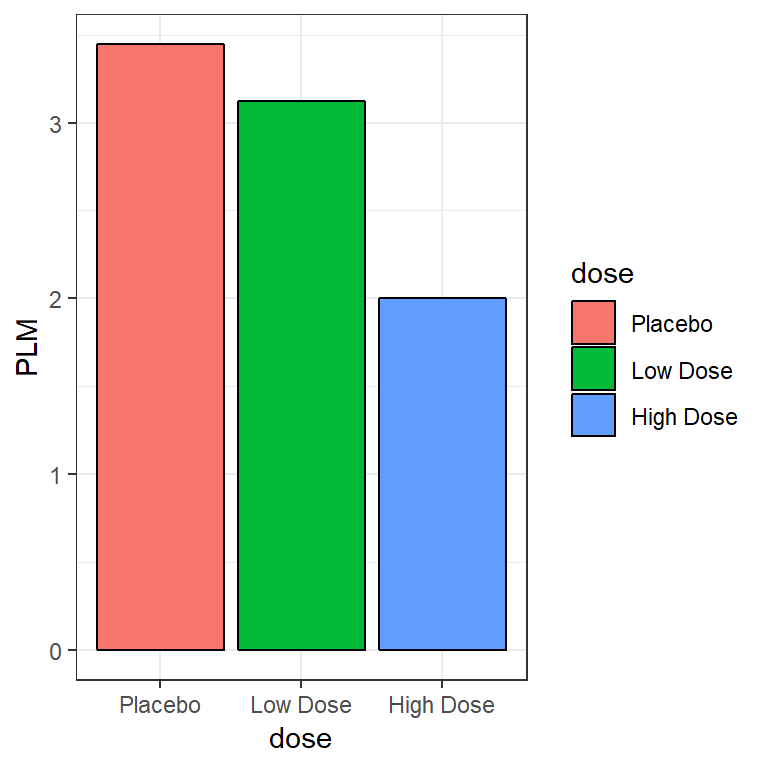
\includegraphics{01_ANCOVA_files/figure-latex/ANCOVA4-1} \end{center}

\begin{verbatim}
## $fill
## [1] FALSE
## 
## attr(,"class")
## [1] "guides"
\end{verbatim}

Bei den Koeffizienten (Estimate) des Modells entspricht der Intercept
den Mittelwert der ersten Dosierungsstufe (= Placebo) und die weiteren
den jeweiligen Abstand zum Mittelwert der Placebodosierung!

\subsubsection*{Berechnung ANCOVA}\label{berechnung-ancova}
\addcontentsline{toc}{subsubsection}{Berechnung ANCOVA}

Nach Überprüfung der Voraussetzungen können wir die ANCOVA berechnen.

\begin{longtable}[]{@{}ccccc@{}}
\caption{Anova Table (Type III tests)}\tabularnewline
\toprule
\begin{minipage}[b]{0.24\columnwidth}\centering\strut
~\strut
\end{minipage} & \begin{minipage}[b]{0.11\columnwidth}\centering\strut
Sum Sq\strut
\end{minipage} & \begin{minipage}[b]{0.06\columnwidth}\centering\strut
Df\strut
\end{minipage} & \begin{minipage}[b]{0.12\columnwidth}\centering\strut
F value\strut
\end{minipage} & \begin{minipage}[b]{0.12\columnwidth}\centering\strut
Pr(\textgreater{}F)\strut
\end{minipage}\tabularnewline
\midrule
\endfirsthead
\toprule
\begin{minipage}[b]{0.24\columnwidth}\centering\strut
~\strut
\end{minipage} & \begin{minipage}[b]{0.11\columnwidth}\centering\strut
Sum Sq\strut
\end{minipage} & \begin{minipage}[b]{0.06\columnwidth}\centering\strut
Df\strut
\end{minipage} & \begin{minipage}[b]{0.12\columnwidth}\centering\strut
F value\strut
\end{minipage} & \begin{minipage}[b]{0.12\columnwidth}\centering\strut
Pr(\textgreater{}F)\strut
\end{minipage}\tabularnewline
\midrule
\endhead
\begin{minipage}[t]{0.24\columnwidth}\centering\strut
\textbf{(Intercept)}\strut
\end{minipage} & \begin{minipage}[t]{0.11\columnwidth}\centering\strut
12.94\strut
\end{minipage} & \begin{minipage}[t]{0.06\columnwidth}\centering\strut
1\strut
\end{minipage} & \begin{minipage}[t]{0.12\columnwidth}\centering\strut
4.257\strut
\end{minipage} & \begin{minipage}[t]{0.12\columnwidth}\centering\strut
0.0492\strut
\end{minipage}\tabularnewline
\begin{minipage}[t]{0.24\columnwidth}\centering\strut
\textbf{partnerLibido}\strut
\end{minipage} & \begin{minipage}[t]{0.11\columnwidth}\centering\strut
15.08\strut
\end{minipage} & \begin{minipage}[t]{0.06\columnwidth}\centering\strut
1\strut
\end{minipage} & \begin{minipage}[t]{0.12\columnwidth}\centering\strut
4.959\strut
\end{minipage} & \begin{minipage}[t]{0.12\columnwidth}\centering\strut
0.03483\strut
\end{minipage}\tabularnewline
\begin{minipage}[t]{0.24\columnwidth}\centering\strut
\textbf{dose}\strut
\end{minipage} & \begin{minipage}[t]{0.11\columnwidth}\centering\strut
25.19\strut
\end{minipage} & \begin{minipage}[t]{0.06\columnwidth}\centering\strut
2\strut
\end{minipage} & \begin{minipage}[t]{0.12\columnwidth}\centering\strut
4.142\strut
\end{minipage} & \begin{minipage}[t]{0.12\columnwidth}\centering\strut
0.02745\strut
\end{minipage}\tabularnewline
\begin{minipage}[t]{0.24\columnwidth}\centering\strut
\textbf{Residuals}\strut
\end{minipage} & \begin{minipage}[t]{0.11\columnwidth}\centering\strut
79.05\strut
\end{minipage} & \begin{minipage}[t]{0.06\columnwidth}\centering\strut
26\strut
\end{minipage} & \begin{minipage}[t]{0.12\columnwidth}\centering\strut
NA\strut
\end{minipage} & \begin{minipage}[t]{0.12\columnwidth}\centering\strut
NA\strut
\end{minipage}\tabularnewline
\bottomrule
\end{longtable}

Betrachtet man die Signifikanz-Werte, so ist klar, dass die Kovariable
die abhängige Variable signifikant vorhersagt, da
\(F(1,26) = 4.96, p = .035\) ist. Es ist also davon auszugehen, dass der
Libido der Person durch die Libido des Partners beeinflusst wird.

Interessant ist, dass nach Berücksichtigung der Wirkung des Libido's vom
Partners die Wirkung von Viagra signifikant ist
(\(F(2,26) = 4.14, p = .028\)).

Wenn wir das nochmals mit den Ergebnissen einer ANOVA (also ohne
Berücksichtigung der Kovariaten vergleichen), stellen wir fest, dass
durch die Kovariate sich ein nicht signifikantes in ein signifikantes
Ergebnis geändert hat.

\begin{longtable}[]{@{}ccccc@{}}
\caption{Anova Table (Type III tests)}\tabularnewline
\toprule
\begin{minipage}[b]{0.21\columnwidth}\centering\strut
~\strut
\end{minipage} & \begin{minipage}[b]{0.11\columnwidth}\centering\strut
Sum Sq\strut
\end{minipage} & \begin{minipage}[b]{0.06\columnwidth}\centering\strut
Df\strut
\end{minipage} & \begin{minipage}[b]{0.12\columnwidth}\centering\strut
F value\strut
\end{minipage} & \begin{minipage}[b]{0.13\columnwidth}\centering\strut
Pr(\textgreater{}F)\strut
\end{minipage}\tabularnewline
\midrule
\endfirsthead
\toprule
\begin{minipage}[b]{0.21\columnwidth}\centering\strut
~\strut
\end{minipage} & \begin{minipage}[b]{0.11\columnwidth}\centering\strut
Sum Sq\strut
\end{minipage} & \begin{minipage}[b]{0.06\columnwidth}\centering\strut
Df\strut
\end{minipage} & \begin{minipage}[b]{0.12\columnwidth}\centering\strut
F value\strut
\end{minipage} & \begin{minipage}[b]{0.13\columnwidth}\centering\strut
Pr(\textgreater{}F)\strut
\end{minipage}\tabularnewline
\midrule
\endhead
\begin{minipage}[t]{0.21\columnwidth}\centering\strut
\textbf{(Intercept)}\strut
\end{minipage} & \begin{minipage}[t]{0.11\columnwidth}\centering\strut
93.44\strut
\end{minipage} & \begin{minipage}[t]{0.06\columnwidth}\centering\strut
1\strut
\end{minipage} & \begin{minipage}[t]{0.12\columnwidth}\centering\strut
26.81\strut
\end{minipage} & \begin{minipage}[t]{0.13\columnwidth}\centering\strut
1.891e-05\strut
\end{minipage}\tabularnewline
\begin{minipage}[t]{0.21\columnwidth}\centering\strut
\textbf{dose}\strut
\end{minipage} & \begin{minipage}[t]{0.11\columnwidth}\centering\strut
16.84\strut
\end{minipage} & \begin{minipage}[t]{0.06\columnwidth}\centering\strut
2\strut
\end{minipage} & \begin{minipage}[t]{0.12\columnwidth}\centering\strut
2.416\strut
\end{minipage} & \begin{minipage}[t]{0.13\columnwidth}\centering\strut
0.1083\strut
\end{minipage}\tabularnewline
\begin{minipage}[t]{0.21\columnwidth}\centering\strut
\textbf{Residuals}\strut
\end{minipage} & \begin{minipage}[t]{0.11\columnwidth}\centering\strut
94.12\strut
\end{minipage} & \begin{minipage}[t]{0.06\columnwidth}\centering\strut
27\strut
\end{minipage} & \begin{minipage}[t]{0.12\columnwidth}\centering\strut
NA\strut
\end{minipage} & \begin{minipage}[t]{0.13\columnwidth}\centering\strut
NA\strut
\end{minipage}\tabularnewline
\bottomrule
\end{longtable}

\begin{longtable}[]{@{}ccccc@{}}
\toprule
\begin{minipage}[b]{0.24\columnwidth}\centering\strut
~\strut
\end{minipage} & \begin{minipage}[b]{0.13\columnwidth}\centering\strut
Estimate\strut
\end{minipage} & \begin{minipage}[b]{0.16\columnwidth}\centering\strut
Std. Error\strut
\end{minipage} & \begin{minipage}[b]{0.12\columnwidth}\centering\strut
t value\strut
\end{minipage} & \begin{minipage}[b]{0.12\columnwidth}\centering\strut
Pr(\textgreater{}\textbar{}t\textbar{})\strut
\end{minipage}\tabularnewline
\midrule
\endhead
\begin{minipage}[t]{0.24\columnwidth}\centering\strut
\textbf{(Intercept)}\strut
\end{minipage} & \begin{minipage}[t]{0.13\columnwidth}\centering\strut
1.789\strut
\end{minipage} & \begin{minipage}[t]{0.16\columnwidth}\centering\strut
0.8671\strut
\end{minipage} & \begin{minipage}[t]{0.12\columnwidth}\centering\strut
2.063\strut
\end{minipage} & \begin{minipage}[t]{0.12\columnwidth}\centering\strut
0.0492\strut
\end{minipage}\tabularnewline
\begin{minipage}[t]{0.24\columnwidth}\centering\strut
\textbf{partnerLibido}\strut
\end{minipage} & \begin{minipage}[t]{0.13\columnwidth}\centering\strut
0.416\strut
\end{minipage} & \begin{minipage}[t]{0.16\columnwidth}\centering\strut
0.1868\strut
\end{minipage} & \begin{minipage}[t]{0.12\columnwidth}\centering\strut
2.227\strut
\end{minipage} & \begin{minipage}[t]{0.12\columnwidth}\centering\strut
0.03483\strut
\end{minipage}\tabularnewline
\begin{minipage}[t]{0.24\columnwidth}\centering\strut
\textbf{doseLow Dose}\strut
\end{minipage} & \begin{minipage}[t]{0.13\columnwidth}\centering\strut
1.786\strut
\end{minipage} & \begin{minipage}[t]{0.16\columnwidth}\centering\strut
0.8494\strut
\end{minipage} & \begin{minipage}[t]{0.12\columnwidth}\centering\strut
2.102\strut
\end{minipage} & \begin{minipage}[t]{0.12\columnwidth}\centering\strut
0.04535\strut
\end{minipage}\tabularnewline
\begin{minipage}[t]{0.24\columnwidth}\centering\strut
\textbf{doseHigh Dose}\strut
\end{minipage} & \begin{minipage}[t]{0.13\columnwidth}\centering\strut
2.225\strut
\end{minipage} & \begin{minipage}[t]{0.16\columnwidth}\centering\strut
0.8028\strut
\end{minipage} & \begin{minipage}[t]{0.12\columnwidth}\centering\strut
2.771\strut
\end{minipage} & \begin{minipage}[t]{0.12\columnwidth}\centering\strut
0.01018\strut
\end{minipage}\tabularnewline
\bottomrule
\end{longtable}

\begin{longtable}[]{@{}cccc@{}}
\caption{Fitting linear model: libido \textasciitilde{} partnerLibido +
dose}\tabularnewline
\toprule
\begin{minipage}[b]{0.18\columnwidth}\centering\strut
Observations\strut
\end{minipage} & \begin{minipage}[b]{0.27\columnwidth}\centering\strut
Residual Std. Error\strut
\end{minipage} & \begin{minipage}[b]{0.11\columnwidth}\centering\strut
\(R^2\)\strut
\end{minipage} & \begin{minipage}[b]{0.20\columnwidth}\centering\strut
Adjusted \(R^2\)\strut
\end{minipage}\tabularnewline
\midrule
\endfirsthead
\toprule
\begin{minipage}[b]{0.18\columnwidth}\centering\strut
Observations\strut
\end{minipage} & \begin{minipage}[b]{0.27\columnwidth}\centering\strut
Residual Std. Error\strut
\end{minipage} & \begin{minipage}[b]{0.11\columnwidth}\centering\strut
\(R^2\)\strut
\end{minipage} & \begin{minipage}[b]{0.20\columnwidth}\centering\strut
Adjusted \(R^2\)\strut
\end{minipage}\tabularnewline
\midrule
\endhead
\begin{minipage}[t]{0.18\columnwidth}\centering\strut
30\strut
\end{minipage} & \begin{minipage}[t]{0.27\columnwidth}\centering\strut
1.744\strut
\end{minipage} & \begin{minipage}[t]{0.11\columnwidth}\centering\strut
0.2876\strut
\end{minipage} & \begin{minipage}[t]{0.20\columnwidth}\centering\strut
0.2055\strut
\end{minipage}\tabularnewline
\bottomrule
\end{longtable}

\subsubsection*{Interpretation ANCOVA}\label{interpretation-ancova}
\addcontentsline{toc}{subsubsection}{Interpretation ANCOVA}

Es scheint ziemlich klar zu sein, dass die signifikante ANOVA einen
Unterschied zwischen der Placebogruppe und den beiden experimentellen
Gruppen widerspiegelt.

\begin{longtable}[]{@{}ccccc@{}}
\caption{Anova Table (Type III tests)}\tabularnewline
\toprule
\begin{minipage}[b]{0.24\columnwidth}\centering\strut
~\strut
\end{minipage} & \begin{minipage}[b]{0.11\columnwidth}\centering\strut
Sum Sq\strut
\end{minipage} & \begin{minipage}[b]{0.06\columnwidth}\centering\strut
Df\strut
\end{minipage} & \begin{minipage}[b]{0.12\columnwidth}\centering\strut
F value\strut
\end{minipage} & \begin{minipage}[b]{0.13\columnwidth}\centering\strut
Pr(\textgreater{}F)\strut
\end{minipage}\tabularnewline
\midrule
\endfirsthead
\toprule
\begin{minipage}[b]{0.24\columnwidth}\centering\strut
~\strut
\end{minipage} & \begin{minipage}[b]{0.11\columnwidth}\centering\strut
Sum Sq\strut
\end{minipage} & \begin{minipage}[b]{0.06\columnwidth}\centering\strut
Df\strut
\end{minipage} & \begin{minipage}[b]{0.12\columnwidth}\centering\strut
F value\strut
\end{minipage} & \begin{minipage}[b]{0.13\columnwidth}\centering\strut
Pr(\textgreater{}F)\strut
\end{minipage}\tabularnewline
\midrule
\endhead
\begin{minipage}[t]{0.24\columnwidth}\centering\strut
\textbf{(Intercept)}\strut
\end{minipage} & \begin{minipage}[t]{0.11\columnwidth}\centering\strut
76.07\strut
\end{minipage} & \begin{minipage}[t]{0.06\columnwidth}\centering\strut
1\strut
\end{minipage} & \begin{minipage}[t]{0.12\columnwidth}\centering\strut
25.02\strut
\end{minipage} & \begin{minipage}[t]{0.13\columnwidth}\centering\strut
3.342e-05\strut
\end{minipage}\tabularnewline
\begin{minipage}[t]{0.24\columnwidth}\centering\strut
\textbf{partnerLibido}\strut
\end{minipage} & \begin{minipage}[t]{0.11\columnwidth}\centering\strut
15.08\strut
\end{minipage} & \begin{minipage}[t]{0.06\columnwidth}\centering\strut
1\strut
\end{minipage} & \begin{minipage}[t]{0.12\columnwidth}\centering\strut
4.959\strut
\end{minipage} & \begin{minipage}[t]{0.13\columnwidth}\centering\strut
0.03483\strut
\end{minipage}\tabularnewline
\begin{minipage}[t]{0.24\columnwidth}\centering\strut
\textbf{dose}\strut
\end{minipage} & \begin{minipage}[t]{0.11\columnwidth}\centering\strut
25.19\strut
\end{minipage} & \begin{minipage}[t]{0.06\columnwidth}\centering\strut
2\strut
\end{minipage} & \begin{minipage}[t]{0.12\columnwidth}\centering\strut
4.142\strut
\end{minipage} & \begin{minipage}[t]{0.13\columnwidth}\centering\strut
0.02745\strut
\end{minipage}\tabularnewline
\begin{minipage}[t]{0.24\columnwidth}\centering\strut
\textbf{Residuals}\strut
\end{minipage} & \begin{minipage}[t]{0.11\columnwidth}\centering\strut
79.05\strut
\end{minipage} & \begin{minipage}[t]{0.06\columnwidth}\centering\strut
26\strut
\end{minipage} & \begin{minipage}[t]{0.12\columnwidth}\centering\strut
NA\strut
\end{minipage} & \begin{minipage}[t]{0.13\columnwidth}\centering\strut
NA\strut
\end{minipage}\tabularnewline
\bottomrule
\end{longtable}

Dieser Effekt kann damit begründet werden, da niedrig- und hochdosierten
Gruppen sehr ähnliche Mittel haben (\(\bar{x}_{Low} = 4.88\),
\(\bar{x}_{High} = 4.85\), während der Mittelwert der Placebogruppe bei
\(\bar{x}_{Placebo} = 3.22\) viel niedriger ist.

\begin{longtable}[]{@{}cccc@{}}
\toprule
\begin{minipage}[b]{0.20\columnwidth}\centering\strut
~\strut
\end{minipage} & \begin{minipage}[b]{0.11\columnwidth}\centering\strut
Libido\strut
\end{minipage} & \begin{minipage}[b]{0.21\columnwidth}\centering\strut
Libido\_Partner\strut
\end{minipage} & \begin{minipage}[b]{0.15\columnwidth}\centering\strut
Libido\_Adj\strut
\end{minipage}\tabularnewline
\midrule
\endhead
\begin{minipage}[t]{0.20\columnwidth}\centering\strut
\textbf{Placebo}\strut
\end{minipage} & \begin{minipage}[t]{0.11\columnwidth}\centering\strut
3.222\strut
\end{minipage} & \begin{minipage}[t]{0.21\columnwidth}\centering\strut
3.444\strut
\end{minipage} & \begin{minipage}[t]{0.15\columnwidth}\centering\strut
2.926\strut
\end{minipage}\tabularnewline
\begin{minipage}[t]{0.20\columnwidth}\centering\strut
\textbf{Low Dose}\strut
\end{minipage} & \begin{minipage}[t]{0.11\columnwidth}\centering\strut
4.875\strut
\end{minipage} & \begin{minipage}[t]{0.21\columnwidth}\centering\strut
3.125\strut
\end{minipage} & \begin{minipage}[t]{0.15\columnwidth}\centering\strut
4.712\strut
\end{minipage}\tabularnewline
\begin{minipage}[t]{0.20\columnwidth}\centering\strut
\textbf{High Dose}\strut
\end{minipage} & \begin{minipage}[t]{0.11\columnwidth}\centering\strut
4.846\strut
\end{minipage} & \begin{minipage}[t]{0.21\columnwidth}\centering\strut
2\strut
\end{minipage} & \begin{minipage}[t]{0.15\columnwidth}\centering\strut
5.151\strut
\end{minipage}\tabularnewline
\bottomrule
\end{longtable}

Eigentlich können wir aber diese Gruppenmittel nicht interpretieren, da
sie nicht um den Effekt der Kovarianz bereinigt wurden. Diese
ursprünglichen Mittel sagen uns nichts über die Gruppenunterschiede, die
sich in der signifikanten ANCOVA widerspiegeln! Daher müssen für diesen
Vergleich die um den Effekt der Kovariaten bereinigten Mittelwerte
verwendet werden. Diese sind in obiger Tabelle in Spalte
\emph{Libido\_Adj} angegeben!

\subsubsection*{Geplante Kontraste}\label{geplante-kontraste}
\addcontentsline{toc}{subsubsection}{Geplante Kontraste}

Für die Berechnung von Kontrasten können entweder vordefinierte
Kontrastcodes, oder eigene Kontrastekodierungen angegeben
werden\footnote{für eine Liste vordefinierter Kontraste siehe Literatur.
  Kontraste können sowohl in SPSS wie auch in R durch entsprechende
  Kontrastcodierungen definiert werden. Bei R ist darauf zu achten, dass
  bei orthogonalen Kontrasten die Type III sum of squares verwendet
  wird, da sonst die Quatratsummen für derartige Kontraste nicht
  stimmen!}. In R lässt sich z.B. ein Kontrast durch folgende Eingabe
definieren:

\begin{longtable}[]{@{}ccccc@{}}
\toprule
\begin{minipage}[b]{0.24\columnwidth}\centering\strut
~\strut
\end{minipage} & \begin{minipage}[b]{0.13\columnwidth}\centering\strut
Estimate\strut
\end{minipage} & \begin{minipage}[b]{0.16\columnwidth}\centering\strut
Std. Error\strut
\end{minipage} & \begin{minipage}[b]{0.12\columnwidth}\centering\strut
t value\strut
\end{minipage} & \begin{minipage}[b]{0.13\columnwidth}\centering\strut
Pr(\textgreater{}\textbar{}t\textbar{})\strut
\end{minipage}\tabularnewline
\midrule
\endhead
\begin{minipage}[t]{0.24\columnwidth}\centering\strut
\textbf{(Intercept)}\strut
\end{minipage} & \begin{minipage}[t]{0.13\columnwidth}\centering\strut
3.126\strut
\end{minipage} & \begin{minipage}[t]{0.16\columnwidth}\centering\strut
0.625\strut
\end{minipage} & \begin{minipage}[t]{0.12\columnwidth}\centering\strut
5.002\strut
\end{minipage} & \begin{minipage}[t]{0.13\columnwidth}\centering\strut
3.342e-05\strut
\end{minipage}\tabularnewline
\begin{minipage}[t]{0.24\columnwidth}\centering\strut
\textbf{partnerLibido}\strut
\end{minipage} & \begin{minipage}[t]{0.13\columnwidth}\centering\strut
0.416\strut
\end{minipage} & \begin{minipage}[t]{0.16\columnwidth}\centering\strut
0.1868\strut
\end{minipage} & \begin{minipage}[t]{0.12\columnwidth}\centering\strut
2.227\strut
\end{minipage} & \begin{minipage}[t]{0.13\columnwidth}\centering\strut
0.03483\strut
\end{minipage}\tabularnewline
\begin{minipage}[t]{0.24\columnwidth}\centering\strut
\textbf{dose1}\strut
\end{minipage} & \begin{minipage}[t]{0.13\columnwidth}\centering\strut
0.6684\strut
\end{minipage} & \begin{minipage}[t]{0.16\columnwidth}\centering\strut
0.24\strut
\end{minipage} & \begin{minipage}[t]{0.12\columnwidth}\centering\strut
2.785\strut
\end{minipage} & \begin{minipage}[t]{0.13\columnwidth}\centering\strut
0.009852\strut
\end{minipage}\tabularnewline
\begin{minipage}[t]{0.24\columnwidth}\centering\strut
\textbf{dose2}\strut
\end{minipage} & \begin{minipage}[t]{0.13\columnwidth}\centering\strut
0.2196\strut
\end{minipage} & \begin{minipage}[t]{0.16\columnwidth}\centering\strut
0.4056\strut
\end{minipage} & \begin{minipage}[t]{0.12\columnwidth}\centering\strut
0.5414\strut
\end{minipage} & \begin{minipage}[t]{0.13\columnwidth}\centering\strut
0.5928\strut
\end{minipage}\tabularnewline
\bottomrule
\end{longtable}

Die Ausgabe des zweiten - oben angegebenen - Kontrastes lässt sich
folgendermaßen interpretieren:

\begin{itemize}
\item
  die erste Variable (\emph{Dosis1}) vergleicht die Placebogruppe mit
  der Niedrig- und Hochdosisgruppe. Als solches vergleicht es den
  angepassten Mittelwert der Placebogruppe
  (\(\bar{x}_{Placebo} = 2.93\)) mit dem Durchschnitt der angepassten
  Mittelwerte für die niedrig- und hochdosierten Gruppen
  (\((4.71+5.15)/2 = 4.93\)).
\item
  der b-Wert für die erste Variable sollte daher die Differenz zwischen
  diesen Werten sein: \(4.93 - 2.93 = 2\).
\item
  dieser Wert wird durch die Anzahl der Gruppen innerhalb des Kontrastes
  (d.h. 3) dividiert und somit \(2/3 = .67\) (wie in der Ausgabe)
  beträgt. Die zugehörige \(t\)-Statistik ist signifikant, was darauf
  hindeutet, dass sich die Placebogruppe signifikant vom kombinierten
  Mittelwert der Viagra-Gruppen unterschied.
\item
  die zweite Variable (\emph{Dosis2}) vergleicht die niedrig- und
  hochdosierten Gruppen, so dass der \(b\)-Wert die Differenz zwischen
  den eingestellten Mitteln dieser Gruppen sein sollte:
  \(5.15 - 4.71 = 0.44\). Dieser Wert wird durch die Anzahl der Gruppen
  innerhalb des Kontrastes (d.h. 2) dividiert wird und somit
  \(0,44/2 = 0,22\) (wie in der Ausgabe) beträgt.
\item
  die zugehörige \(t\)-Statistik ist nicht signifikant (\(p = .590\)),
  was darauf hindeutet, dass die hochdosierte Gruppe keine signifikant
  höhere Libido produzierte als die niedrigdosierte Gruppe.
\item
  der Wert für die \emph{Kovariable} beträgt (\(b = 0.416\)). Wenn also
  der Libido eines Partners um eine Einheit zunimmt, sollte der Libido
  der Person um knapp eine halbe Einheit zunehmen (obwohl es nichts
  gibt, was auf einen kausalen Zusammenhang zwischen den beiden
  hinweist).
\item
  das Vorzeichen dieses Koeffizienten zeigt in welche Richtung die
  Beziehung zwischen der Kovariablen und dem Ergebnis geht. Da der
  Koeffizient in diesem Beispiel positiv ist, bedeutet dies also, dass
  die Libido des Partners in einem positiven Verhältnis zur Libido des
  Teilnehmers steht:
\item
  mit dem einen steigt auch der andere.
\item
  ein negativer Koeffizient würde das Gegenteil bedeuten: wenn einer
  steigt, sinkt der andere.
\end{itemize}

\subsubsection*{Interpretation
Kovariate}\label{interpretation-kovariate}
\addcontentsline{toc}{subsubsection}{Interpretation Kovariate}

Für die Interpretatiom der Kovariaten verwendet man am besten die
Parameterschätzungen (\(b\)) in folgender Weise:

\begin{itemize}
\tightlist
\item
  wenn der \(b\)-Wert für die Kovariable positiv ist, haben die
  Kovariable und die Ergebnisvariable eine positive Beziehun, also mit
  zunehmenden Werten der Kovariable steigt auch das Ergebnis!
\item
  wenn der \(b\)-Wert negativ ist, bedeutet das das Gegenteil.
\end{itemize}

Für diese Daten war der \(b\)-Wert positiv, was darauf hindeutet, dass
mit zunehmender Libido des Partners auch die Libido des Teilnehmers
steigt. Eine weitere Möglichkeit, das Gleiche zu entdecken, besteht
darin, einfach einen Streudiagramm der Kovariablen gegen das Ergebnis zu
zeichnen.

Abschließend wird durch den Scatterplot nochmals bestätigt, was wir
bereits wissen: die Kovariable bewirkt, dass mit zunehmender
Partnerlibido auch die Libido des Teilnehmers zunimmt (wie die Steigung
der Regressionslinie zeigt).

\begin{center}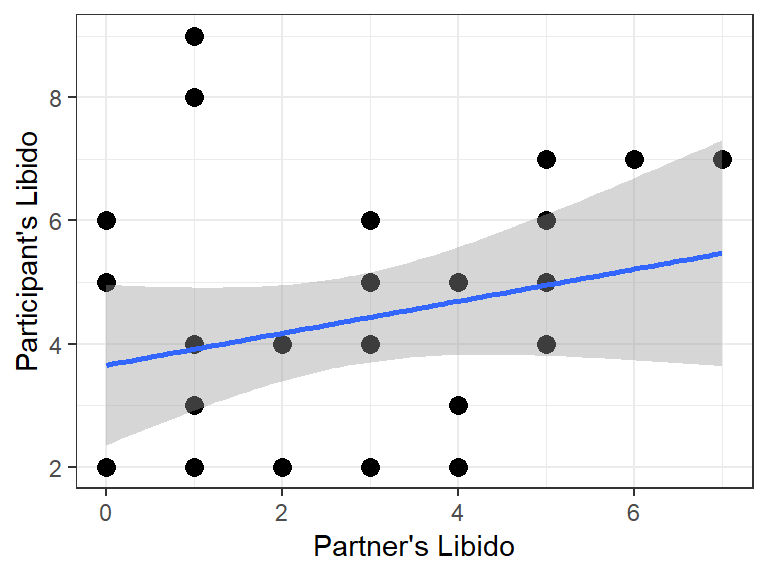
\includegraphics{01_ANCOVA_files/figure-latex/ANCOVA10-1} \end{center}

\subsubsection*{Post hoc Tests}\label{post-hoc-tests}
\addcontentsline{toc}{subsubsection}{Post hoc Tests}

Wie bereits aus der ANOVA bekannt sein sollte, werden bei den Post hoc
Tests alle Stufen der unabhängigen Variablen paarweise miteinander
verglichen. Im Unterschied zur herkömmlichen ANOVA weden jedoch bei der
ANCOVA die adjustierten Mittelwerte verwendet!

Das Ergebnis zeigt die drei Vergleiche (niedrige Dosis vs.~Placebo, hohe
Dosis vs.~Placebo, hohe Dosis vs.~niedrige Dosis).

Verglichen werden die Differenzen zu den adjustierten Gruppenmitteln

\begin{itemize}
\tightlist
\item
  die Schätzung für die niedrige Dosis vs.~Placebo beträgt
  \(4.71 - 2.93 = 1.78\)
\item
  für die hohe Dosis vs.~Placebo beträgt sie \(5.15 - 2.93 = 2.22\) und
\item
  für die niedrige vs.~hohe \(5.15 - 4.71 = 0.44\)
\end{itemize}

Der angegebene Standardfehler bezieht sich auf die Differenz zwischen
den adjusiterten Mittelwerten.

Der \(t\)-Test (Differenz zwischen den Mitteln geteilt durch den
Standardfehler) und dem zugehörigen \(p\)-Wert deutet auf signifikante
Unterschiede zwischen der Hochdosis- und Placebogruppe
(\(t = 2.77, p < .050\)) hin.

Kein Unterschied besteht zwischen der Niedrigdosisgruppe und der
Placebogruppe (\(t = 2.10, p = .120\)) und der Hochdosisgruppe
(\(t = 0.54, p = .850\)).

Die Konfidenzintervalle bestätigen diese Schlussfolgerung (weil sie für
den Vergleich der Hochdosis- und Placebogruppen Null nicht enthalten).

\begin{verbatim}
## 
##   Simultaneous Tests for General Linear Hypotheses
## 
## Multiple Comparisons of Means: Tukey Contrasts
## 
## 
## Fit: aov(formula = libido ~ partnerLibido + dose, data = viagraData)
## 
## Linear Hypotheses:
##                           Estimate Std. Error t value Pr(>|t|)  
## Low Dose - Placebo == 0      1.786      0.849    2.10    0.109  
## High Dose - Placebo == 0     2.225      0.803    2.77    0.027 *
## High Dose - Low Dose == 0    0.439      0.811    0.54    0.852  
## ---
## Signif. codes:  0 '***' 0.001 '**' 0.01 '*' 0.05 '.' 0.1 ' ' 1
## (Adjusted p values reported -- single-step method)
\end{verbatim}

\begin{verbatim}
## 
##   Simultaneous Confidence Intervals
## 
## Multiple Comparisons of Means: Tukey Contrasts
## 
## 
## Fit: aov(formula = libido ~ partnerLibido + dose, data = viagraData)
## 
## Quantile = 2.48
## 95% family-wise confidence level
##  
## 
## Linear Hypotheses:
##                           Estimate lwr    upr   
## Low Dose - Placebo == 0    1.786   -0.324  3.895
## High Dose - Placebo == 0   2.225    0.231  4.219
## High Dose - Low Dose == 0  0.439   -1.575  2.454
\end{verbatim}

\subsection*{Nützliche Graphen}\label{nutzliche-graphen}
\addcontentsline{toc}{subsection}{Nützliche Graphen}

Zur Überprüfung von Voraussetzungen können sich folgende Graphiken als
hilfreich erweisen:

\begin{center}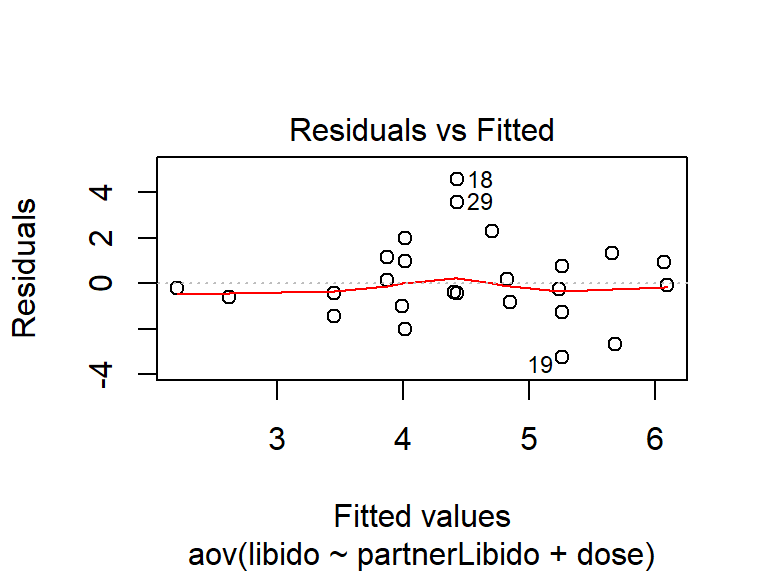
\includegraphics{01_ANCOVA_files/figure-latex/ANCOVA13-1} \end{center}

\begin{center}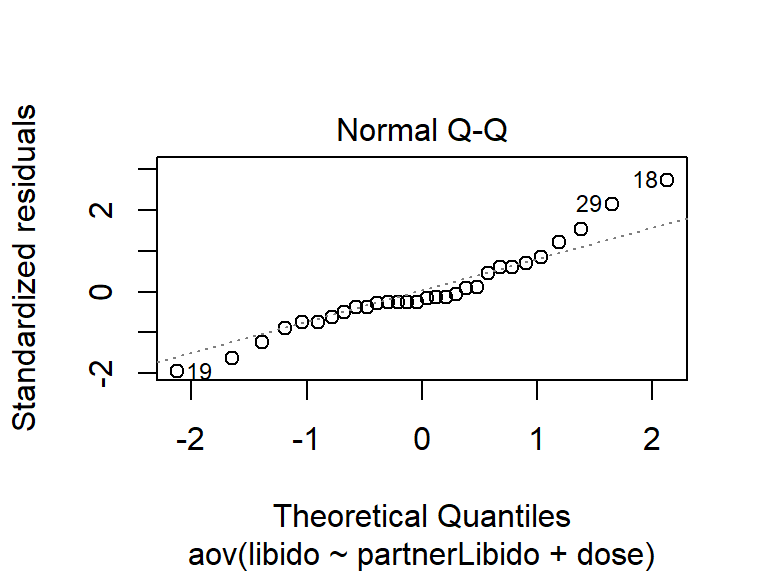
\includegraphics{01_ANCOVA_files/figure-latex/ANCOVA13-2} \end{center}

\begin{center}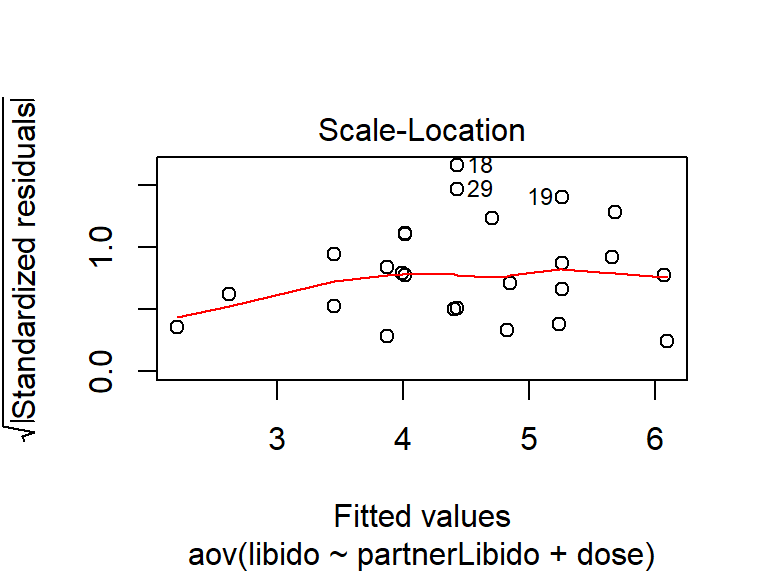
\includegraphics{01_ANCOVA_files/figure-latex/ANCOVA13-3} \end{center}

\begin{center}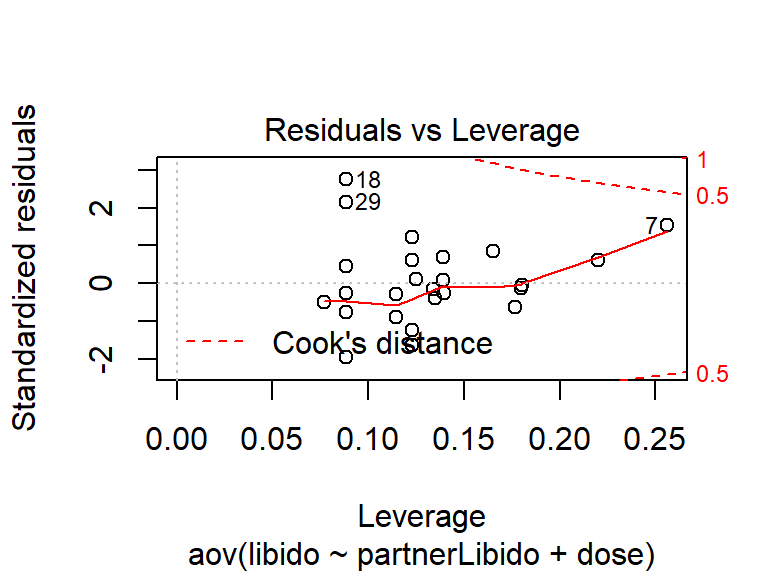
\includegraphics{01_ANCOVA_files/figure-latex/ANCOVA13-4} \end{center}

Von den vier Diagramme sind die ersten beiden die wichtigsten:

\begin{itemize}
\tightlist
\item
  Ersterer kann zur Überprüfung der Varianzhomogenität der Varianz
  verwendet werden. Es zeigt sich, dass die Verteilung der Scores an
  einigen Stellen breiter als an anderenis (Funnelling). Die Residuen
  sind also heteroscedastisch.
\item
  Das zweite Diagramm ist ein Q-Q-Diagramm. Die Punkte im Diagramm
  sollten nahe der diagonalen Linie liegen. Die vorliegende Verteilung
  deutet darauf hin, dass keine Normalverteilung vorliegt und daher eher
  eine robuste ANCOVA\footnote{robuste ANCOVAS werden in dieser LV nicht
    näher besprochen - siehe Literatur.} angebracht wäre.
\item
  Die dritte Graphik wird auch als \emph{Spread-Location-Plot}
  bezeichnet. Diese Darstellung zeigt, ob die Residuen gleichmäßig über
  die Bereiche der Prädiktoren verteilt sind. So können Sie die Annahme
  der gleichen Varianz (Homoscedastizität) überprüfen. Es ist gut, wenn
  man eine horizontale Linie mit gleichmäßig (zufällig) gespreizten
  Punkten sehen - was hier nicht der Fall ist.
\item
  Die vierte Graphik identifiziert einflussreiche Fälle (Ausreißer).
  Nicht alle Ausreißer beeinflussen die linearen Regressionsanalyse im
  negativen Sinn, d.h. die Ergebnisse wären nicht viel anders, wenn wir
  sie entweder einbeziehen oder von der Analyse ausschließen würden. Sie
  folgen in den meisten Fällen dem Trend und sind nicht wirklich
  wichtig. Andererseits können einige Fälle sehr einflussreich sein,
  auch wenn sie sich in einem angemessenen Bereich der Werte bewegen.
  Sie können Extremfälle gegen eine Regressionslinie sein und die
  Ergebnisse verändern, wenn wir sie von der Analyse ausschließen. Im
  Gegensatz zu den anderen Graphiken sind hier Muster nicht relevant.
  Man achtet auf die äußeren Werte in der oberen rechten Ecke oder in
  der unteren rechten Ecke. Diese Punkte sind die Orte, an die für eine
  Regressionslinie einflussreich sein können. Man beachtet vor allem
  Fälle, die \emph{außerhalb einer gestrichelten Linie} (Cook's
  Distance) sind. Werte die außerhalb liegen, sind für die
  Regressionsergebnisse von Bedeutung. Die Regressionsergebnisse werden
  geändert, wenn wir diese Fälle ausschließen!
\end{itemize}

\subsection*{Homogenität der Steigung}\label{homogenitat-der-steigung}
\addcontentsline{toc}{subsection}{Homogenität der Steigung}

Bereits im Scatterplot der nach Gruppen getrennten Regressionen konnten
wir feststellen, dass die Annahme der Homogenität der
Regressionssteigungen für die \emph{Hochdosisgruppe} unterschiedlich
verletzt wird. Um einen statistischen Test dieser Annahme durchzufürhen,
wird die ANCOVA unter Einbeziehung des Interaktionseffektes zwischen der
Kovariaten und dem Prädiktor nochmals durchgeführt.

\begin{longtable}[]{@{}ccccc@{}}
\caption{Anova Table (Type III tests)}\tabularnewline
\toprule
\begin{minipage}[b]{0.30\columnwidth}\centering\strut
~\strut
\end{minipage} & \begin{minipage}[b]{0.11\columnwidth}\centering\strut
Sum Sq\strut
\end{minipage} & \begin{minipage}[b]{0.06\columnwidth}\centering\strut
Df\strut
\end{minipage} & \begin{minipage}[b]{0.12\columnwidth}\centering\strut
F value\strut
\end{minipage} & \begin{minipage}[b]{0.13\columnwidth}\centering\strut
Pr(\textgreater{}F)\strut
\end{minipage}\tabularnewline
\midrule
\endfirsthead
\toprule
\begin{minipage}[b]{0.30\columnwidth}\centering\strut
~\strut
\end{minipage} & \begin{minipage}[b]{0.11\columnwidth}\centering\strut
Sum Sq\strut
\end{minipage} & \begin{minipage}[b]{0.06\columnwidth}\centering\strut
Df\strut
\end{minipage} & \begin{minipage}[b]{0.12\columnwidth}\centering\strut
F value\strut
\end{minipage} & \begin{minipage}[b]{0.13\columnwidth}\centering\strut
Pr(\textgreater{}F)\strut
\end{minipage}\tabularnewline
\midrule
\endhead
\begin{minipage}[t]{0.30\columnwidth}\centering\strut
\textbf{(Intercept)}\strut
\end{minipage} & \begin{minipage}[t]{0.11\columnwidth}\centering\strut
53.54\strut
\end{minipage} & \begin{minipage}[t]{0.06\columnwidth}\centering\strut
1\strut
\end{minipage} & \begin{minipage}[t]{0.12\columnwidth}\centering\strut
21.92\strut
\end{minipage} & \begin{minipage}[t]{0.13\columnwidth}\centering\strut
9.323e-05\strut
\end{minipage}\tabularnewline
\begin{minipage}[t]{0.30\columnwidth}\centering\strut
\textbf{partnerLibido}\strut
\end{minipage} & \begin{minipage}[t]{0.11\columnwidth}\centering\strut
17.18\strut
\end{minipage} & \begin{minipage}[t]{0.06\columnwidth}\centering\strut
1\strut
\end{minipage} & \begin{minipage}[t]{0.12\columnwidth}\centering\strut
7.035\strut
\end{minipage} & \begin{minipage}[t]{0.13\columnwidth}\centering\strut
0.01395\strut
\end{minipage}\tabularnewline
\begin{minipage}[t]{0.30\columnwidth}\centering\strut
\textbf{dose}\strut
\end{minipage} & \begin{minipage}[t]{0.11\columnwidth}\centering\strut
36.56\strut
\end{minipage} & \begin{minipage}[t]{0.06\columnwidth}\centering\strut
2\strut
\end{minipage} & \begin{minipage}[t]{0.12\columnwidth}\centering\strut
7.484\strut
\end{minipage} & \begin{minipage}[t]{0.13\columnwidth}\centering\strut
0.00298\strut
\end{minipage}\tabularnewline
\begin{minipage}[t]{0.30\columnwidth}\centering\strut
\textbf{partnerLibido:dose}\strut
\end{minipage} & \begin{minipage}[t]{0.11\columnwidth}\centering\strut
20.43\strut
\end{minipage} & \begin{minipage}[t]{0.06\columnwidth}\centering\strut
2\strut
\end{minipage} & \begin{minipage}[t]{0.12\columnwidth}\centering\strut
4.181\strut
\end{minipage} & \begin{minipage}[t]{0.13\columnwidth}\centering\strut
0.02767\strut
\end{minipage}\tabularnewline
\begin{minipage}[t]{0.30\columnwidth}\centering\strut
\textbf{Residuals}\strut
\end{minipage} & \begin{minipage}[t]{0.11\columnwidth}\centering\strut
58.62\strut
\end{minipage} & \begin{minipage}[t]{0.06\columnwidth}\centering\strut
24\strut
\end{minipage} & \begin{minipage}[t]{0.12\columnwidth}\centering\strut
NA\strut
\end{minipage} & \begin{minipage}[t]{0.13\columnwidth}\centering\strut
NA\strut
\end{minipage}\tabularnewline
\bottomrule
\end{longtable}

Die Auswirkungen der Dosis von Viagra und der Libido des Partners sind
immer noch signifikant, aber da die Interaktion (partnerLibido:dose)
signifikant (\(p = .028\)) ist, ist die Annahme der Homogenität der
Regressionsgeraden verletzt.

Obwohl dieser Befund nicht überraschend ist (vgl. Graphik oben), gibt er
Anlass zur Sorge über die Hauptanalyse. Dieses Beispiel veranschaulicht,
warum es wichtig ist, Annahmen zu testen und nicht nur die Ergebnisse
einer Analyse blind zu akzeptieren!

\subsection*{Bericht der Ergebnisse}\label{bericht-der-ergebnisse}
\addcontentsline{toc}{subsection}{Bericht der Ergebnisse}

Der Ergebnissbericht einer ANCOVA ist weitgehend identisch mit der einer
ANOVA. Hinzu kommt lediglich die Wirkung der Kovariablen. Für die
Kovariable und den experimentellen Effekt berichten wir Details über das
\(F\)-Verhältnis und die Freiheitsgrade, aus denen es berechnet wurde.
In beiden Fällen wurde das \(F\)-Verhältnis aus der Division der
mittleren Quadrate für den Effekt durch die mittleren Quadrate der
Residuen ermittelt. Die Freiheitsgrade zur Beurteilung des \(F\)-Wertes
sind daher die Freiheitsgrade für die Wirkung des Modells (\(df_M = 1\)
für die Kovariable und \(2\) für die experimentelle Wirkung) und die
Freiheitsgrade für die Residuen des Modells (\(df_R = 26\) für die
Kovariable und die experimentelle Wirkung). Der Bericht könnte
folgendermaßen abgefasst werden:

\begin{quote}
Die Kovariable (Libido des Partners) zeigt einen signifikanten
Zusammenhang mit dem Libido des Teilnehmers
(\(F(1, 26) = 4.96, p < .050, r = 0.40\). Kontrolliert man für den
Effelt des Libido's des Partners, dann zeigt sich auch ein signifikanter
Effekt der Dosis von Viagra auf den Libido
(\(F(2, 26) = 4.14, p < .050, \eta^2_{part} = .24\)).
\end{quote}

\begin{quote}
Die geplanten Kontraste zeigten, dass die Einnahme einer hohen oder
niedrigen Dosis von Viagra den Libido im Vergleich zur Einnahme eines
Placebos signifikant erhöht (\(t(26) = 2,79, p < .010, r = 0.48\)). Es
gab keinen signifikanten Unterschied zwischen der hohen und niedrigen
Dosis von Viagra (\(t(26) = 0.54, p = .590, r = 0.11\)).
\end{quote}

\begin{quote}
Die Tukey-Post-Hoc-Tests zeigten, dass der über die Kovariate angepasste
Mittelwert der Hochdosis-Gruppe signifikant größer war als der des
Placebos (Differenz = 2.22, \(t = 2.77, p < .050, d = 1,13\)). Es gab
jedoch keinen signifikanten Unterschied zwischen der Niedrigdosis- und
Placebogruppe (Differenz = 1.79, \(t = 2.10, p = .110, d = 1.04\)) und
zwischen der Niedrigdosis- und der Hochdosisgruppe (Differenz = 0.44,
\(t = 0.54, p = .850, d = 0.11\)).
\end{quote}

\begin{quote}
Trotz der fehlenden Bedeutung zwischen der Niedrigdosis- und der
Placebogruppe war die Effektgröße ziemlich groß.
\end{quote}

\hypertarget{refs}{}
\hypertarget{ref-Buehner1}{}
Bühner, M. 2009. \emph{Statistik Für Psychologen Und
Sozialwissenschaftler}. Erste Auflage. Martin-Kollar-Str. 10-12, D-81829
München/Germany: Pearson Education Deutschland GmbH.

\hypertarget{ref-Buehner2}{}
---------. 2017. \emph{Statistik Für Psychologen Und
Sozialwissenschaftler}. Zweite Auflage. Lilienthalstraße 2, 85399
Hallbergmoos, Germany: Pearson Deutschland GmbH.

\hypertarget{ref-CourseRa}{}
Coursera. 2018. ``Coursera Take the World's Best Courses.''
\url{https://www.coursera.org/}.

\hypertarget{ref-DataCamp}{}
DataCamp. 2018. ``DataCamp Learn Data Science.''
\url{https://www.datacamp.com/}.

\hypertarget{ref-Field}{}
Field, A. 2017. \emph{Discovering Statistics Using R}. 2nd ed. 1 Olivers
Yard, 55 City Road, London EC1Y 1SP: SAGE Publications Ltd.

\hypertarget{ref-Stevens}{}
Stevens, J.P. 2002. ``Applied Multivariate Statistics for the Social
Sciences.'' \emph{APA PsycNET}.

\hypertarget{ref-Wildt}{}
Wildt, A. 2009. \emph{Analysis of Covariance}. 12th ed. 1 Olivers Yard,
55 City Road, London EC1Y 1SP: SAGE Publications Ltd.


\end{document}
